\chapter{连续场}

在第三章中，我们讨论了网格上的数值问题：不论是电路网络，还是被弹簧串在一起的振子，都是一个个离散的系统，相互之间耦合在一起，展现出复杂的行为。在更多时候，现实中所面临的问题会是连续化的：我们需要求解大块导体中的电流流动、从天线辐射出的电磁波，抑或鼓面的振动。这些时候，物理量表现为场：时空的连续函数 $\phi(\bm r,t)$。在数值上，通常会先将连续的时空离散成网格，然后用上一章的办法求解。然而，如何进行离散，如何利用问题的特殊性质在数值上简化，这值得我们在这一章中来详细讨论。

\section{静电静磁：泊松方程的边值问题}

在学习物理的过程中，我们首先接触到的场往往是静电场和静磁场。对于静电场，我们可以引入标量场电势 $\phi(\bm r)$，其满足泊松方程
\begin{equation}
\nabla^2\phi=-\rho/\varepsilon_0.
\tag{5.1.1}
\end{equation}
而对于静磁场，我们也可以在无电流的单连通区域内引入满足拉普拉斯方程的磁标势，不同单连通区域再通过边界条件相连接。

对于这样一个方程，在给定了非齐次项 $\rho$，也就是电荷密度分布后，再加上合适的边界条件，根据唯一性定理就能完全确定 $\phi$ 的全空间分布。这类问题通常称为\textbf{边值问题}。本节中我们将初步探讨如何从数值上求解这类问题。

\subsection{解析求解与打靶法}

我们从一维泊松方程的边值问题出发讨论边值问题的一些基础概念：
\begin{equation}
\begin{cases}
-u''=f(x),\\
u(0)=0,\\
u(1)=0.
\end{cases}
\tag{5.1.2}
\end{equation}
这个问题可以理解成两块接地的平行导体板之间有电荷分布 $f(x)$，求电势 $u(x)$。它能够解析求解。对 (5.1.2) 式两端做一次积分，得到
\begin{equation}
u'(x)=-\int_0^x f(x_1)\,\mathrm dx_1+u'(0),
\tag{5.1.3}
\end{equation}
出现了未知的 $x=0$ 处的导数。再做一次积分，得到
\begin{align}
u(x)&=-\int_0^x\mathrm dx_1\int_0^{x_1}\mathrm dx_2\,f(x_2)+xu'(0)+u(0)\notag\\
&=-\int_0^x(x-x_1)f(x_1)\,\mathrm dx_1+xu'(0)+u(0).
\tag{5.1.4}
\end{align}
代入边界条件 $u(1)=0$，可以解得
\begin{equation}
u'(0)=\int_0^1(1-x)f(x)\,\mathrm dx.
\tag{5.1.5}
\end{equation}
最后得到问题的解
\begin{align}
u(x)&=-\int_0^x(x-x_1)f(x_1)\,\mathrm dx_1+x\int_0^1(1-x_1)f(x_1)\,\mathrm dx_1\notag\\
&=(1-x)\int_0^x x_1f(x_1)\,\mathrm dx_1+x\int_x^1(1-x_1)f(x_1)\,\mathrm dx_1.
\tag{5.1.6}
\end{align}

上述解析演算的过程实际上非常类似于求解一维边值问题中常用的\textbf{打靶法}（shooting method）。我们考虑一个一般的二阶线性微分方程的一维边值问题：
\begin{equation}
\begin{cases}
y''+p(x)y'+q(x)y=f(x),\\
(\alpha_1y+\beta_1y')|_{x_1}=b_1,\\
(\alpha_2y+\beta_2y')|_{x_2}=b_2.
\end{cases}
\tag{5.1.7}
\end{equation}
原则上讲，如果已知一端的初始条件 $y(x_1),y'(x_1)$，我们可以直接将方程改写成初值问题，然后使用先前讨论过的常微分方程的初值问题算法来求解，例如 R--K 算法。但现在是两个端点各给了一个边界条件，我们就需要先从一端开始做一些尝试：
\begin{enumerate}[label=(\arabic*)]
\item 选取一组满足边界点 1 边界条件的函数值和导数值：
\[
\alpha_1g_1(x_1)+\beta_1g_1'(x_1)=b_1.
\]
\item 通过初值问题的数值算法求解后续的函数值 $g_1(x)$。
\item 得到边界点 2 的函数值 $g_1(x_2)$ 和导数值 $g_1'(x_2)$。一般而言它们不满足另一个边界条件，但我们知道由于方程和算法都是线性的，残差
\[
\delta_1=\alpha_2g_1(x_2)+\beta_2g_1'(x_2)-b_2
\]
必然是边界点 1 处函数值和导数值的线性函数。
\item 选取另一组满足边界点 1 边界条件的函数值和导数值，不失一般性地，
\[
 g_2(x_1)=g_1(x_1)+\gamma_0\beta_1,\qquad
 g_2'(x_1)=g_1'(x_1)-\gamma_0\alpha_1.
\]
可相应计算出 $\delta_2=\alpha_2g_2(x_2)+\beta_2g_2'(x_2)-b_2$。
\item 从线性关系可知满足全部边界条件的解应该取 $\gamma=\gamma_0/(1-\delta_2/\delta_1)$，而完整的解为
\begin{equation}
u(x)=\frac{\delta_2g_1(x)-\delta_1g_2(x)}{\delta_2-\delta_1}.
\tag{5.1.8}
\end{equation}
\end{enumerate}
从上面的描述可以看出，我们利用方程的线性，将一个边值问题转换为以不同初始条件两次求解一个初值问题，来得到满足两端点边界条件的解。其名字也暗含了这个寓意：打靶时射击点和靶子都是固定的，而射角可调，利用两次射击得到的数据便可以确定如何射击能够得到一条准确击中目标的轨迹。

事实上，对于非线性边值问题和本征值问题，打靶法依旧适用，但此时需要求一个非线性方程 $\delta(\gamma)=0$ 的根。容易注意到，(5.1.8) 式与 2.4 节中的弦割法完全一致，只不过对于这里的线性方程可以一步求得准确解。对于非线性情形，也可以使用我们在 2.4 节中学过的其余求根方法来解决。

\begin{exerciseBox}[练习 5.1]
用打靶法求解非线性边值问题 $y''=-\delta e^y,\ y(0)=y(1)=0$。检验当参数 $\delta$ 满足 $0<\delta<\delta_c\approx3.51$ 时，该边值问题存在两个解。
\end{exerciseBox}

\subsection{格林函数与有限差分}

我们重新回到原泊松方程的解析解
\begin{equation}
u(x)=(1-x)\int_0^x x_1f(x_1)\,\mathrm dx_1+x\int_x^1(1-x_1)f(x_1)\,\mathrm dx_1.
\tag{5.1.9}
\end{equation}
如果定义函数
\begin{equation}
G(x,s)=
\begin{cases}
(1-x)s,&0\le s\le x,\\
(1-s)x,&x<s\le1,
\end{cases}
\tag{5.1.10}
\end{equation}
那么方程的解可以简化为
\begin{equation}
u(x)=\int_0^1G(x,s)f(s)\,\mathrm ds.
\tag{5.1.11}
\end{equation}
这里，$G(x,s)$ 被称为方程 (5.1.2) 的\textbf{格林函数}。我们容易注意到，格林函数关于变量 $x$ 和 $s$ 是交换对称的，并且在整个定义域上非负且有界，最大值为 $1/4$。据此可以证明如下不等式：
\begin{equation}
\max_x|u(x)|\le\frac14\max_x|f(x)|.
\tag{5.1.12}
\end{equation}
这指出了一维泊松方程的解是有界的。

现在我们暂时不管格林函数，而是考虑求解边值问题的另一个思路：将自变量区间 $[0,1]$ 离散化，用差分近似导数，将微分方程变为线性方程组。具体来说，在定义域 $x\in[0,1]$ 上选取 $n+1$ 个均匀分布的节点 $\{x_i=ih\}_{i=0}^{n}$，其中间隔 $h=1/n$。函数 $u$ 在这些节点上的值简记作 $\{u_i=u(x_i)\}_{i=0}^{n}$。二阶导数可以使用中心差分来近似：
\begin{equation}
u''(x)=\frac{u(x+h)-2u(x)+u(x-h)}{h^2}+O(h^2),
\tag{5.1.13}
\end{equation}
得到方程组
\begin{equation}
\begin{cases}
u_i=0,&i=0,n,\\[3pt]
\displaystyle\frac{-u_{i+1}+2u_i-u_{i-1}}{h^2}=f_i,&i=1,2,\ldots,n-1.
\end{cases}
\tag{5.1.14}
\end{equation}
引入 $\bm u=(u_1,\ldots,u_{n-1})^{\mathrm T},\ \bm f=(f_1,\ldots,f_{n-1})^{\mathrm T}$，得到
\begin{equation}
A\bm u=\bm f,
\tag{5.1.15}
\end{equation}
其中 $A$ 是对角元为 $2/h^2$、次对角元为 $-1/h^2$ 的三对角矩阵。

现在我们通过将微分近似替换为差分，把微分方程的边值问题转换为了一个线性代数方程组的求解问题。差分过程中产生的误差为 $O(h^2)$，我们称该微分方程差分格式的\textbf{局部截断误差}为二阶。显然，使用追赶法可以轻松求解这个三对角矩阵对应的方程组。

我们可以仔细考究一下矩阵 $A$ 的性质。考察二次型
\begin{align}
\bm u^{\mathrm T}A\bm u
&=\frac{2}{h^2}\sum_{i=1}^{n-1}u_i^2-\frac{2}{h^2}\sum_{i=2}^{n-1}u_iu_{i-1}\notag\\
&=\frac1{h^2}\left[u_1^2+u_{n-1}^2+\sum_{i=2}^{n-1}(u_i-u_{i-1})^2\right]\ge0,
\tag{5.1.16}
\end{align}
可知矩阵 $A$ 以及其逆 $A^{-1}$ 都是正定的，与解析的格林函数性质相符合。事实上，我们在第四章的大作业中也见过这个三对角的对称矩阵 $A$，在那里它作为线性弹簧等距平衡的刚度矩阵而存在。我们可以知道 $A$ 的全体本征值
\begin{equation}
\lambda_i=\frac4{h^2}\sin^2\frac{\pi i}{2n}=4n^2\sin^2\frac{\pi i}{2n},\qquad i=1,2,\ldots,n-1,
\tag{5.1.17}
\end{equation}
和相应本征向量（$j$ 表示的是本征向量的各分量）
\begin{equation}
(q_i)_j=\sqrt{\frac2n}\sin\frac{\pi ij}{n},\qquad i,j=1,2,\ldots,n-1.
\tag{5.1.18}
\end{equation}
\jiaokan{原印本将式 (5.1.18) 的归一化因子印为 $\sqrt{2/(n-1)}$。由离散正弦基的正交关系 $\sum_{j=1}^{n-1}\sin(\pi ij/n)\sin(\pi kj/n)=\frac n2\delta_{ik}$，归一化因子应为 $\sqrt{2/n}$。}
根据此关系，我们可以证明
\begin{equation}
\|u\|_2\le\frac{1}{4n^2\sin^2(\pi/2n)}\|f\|_2<\frac1{\pi^2}\|f\|_2.
\tag{5.1.19}
\end{equation}
这个式子相当于说明了算法的稳定性：不论网格怎么取，数值解总是有界的。

如果不去考虑如何解得快，而是写出形式解
\begin{equation}
\bm u=A^{-1}\bm f,
\tag{5.1.20}
\end{equation}
将其与 (5.1.11) 式相对照，我们看到 $A^{-1}$ 这个矩阵似乎和函数算符 $\int G(x,s)[\cdots] \,\mathrm ds$ 的地位相当，只是后者作用在函数 $f(s)$ 上，而前者作用在向量 $\bm f$ 上。进一步地，注意到矩阵乘法就是一个求和操作
\[
u_i=\sum_{j=1}^{n-1}(A^{-1})_{ij}f_j,
\]
这与将 (5.1.11) 式中的积分离散化按梯形法数值积分得到的和式
\begin{equation}
u(x_i)\approx\frac h2\bigl[G(x_i,0)f(0)+G(x_i,1)f(1)\bigr]+h\sum_{j=1}^{n-1}G(x_i,x_j)f(x_j)
\tag{5.1.21}
\end{equation}
在形式上是相同的。因此我们可以将格林函数想象成矩阵形式，定义 $(G)_{ij}=hG(x_i,x_j)$，将积分变为矩阵乘法，我们看到
\begin{align}
(AG)_{ij}
&=\frac{2G_{ij}-G_{i+1,j}-G_{i-1,j}}{h^2}\notag\\
&=\frac1h
\begin{cases}
2(1-x_i)x_j-(1-x_{i+1})x_j-(1-x_i)x_{j-1},& i=j,\\
2(1-x_i)x_j-(1-x_{i+1})x_j-(1-x_{i-1})x_j,& i>j,\\
2(1-x_i)x_j-(1-x_i)x_{j+1}-(1-x_{i-1})x_j,& i<j,
\end{cases}\notag\\
&=\delta_{ij},
\tag{5.1.22}
\end{align}
也就是说 $A^{-1}=G$，即
\begin{equation}
u_i=\sum_{j=1}^{n-1}hG(x_i,x_j)f(x_j).
\tag{5.1.23}
\end{equation}
这意味着有限差分法等价于将用格林函数表示的解析解中的积分用梯形法近似。

有了 (5.1.23) 式，也可以借助 2.2 节中算法 2.2 的结论来得到有限差分法的误差估计：
\begin{equation}
\max_i|u_i-u(x_i)|\le\frac{h^2}{12}\max_{x\in(0,1)}\left|\frac{\mathrm d^2}{\mathrm dx^2}G(x_i,x)f(x)\right|.
\tag{5.1.24}
\end{equation}
即对于一个二阶导数有界的函数 $f(x)$，在取充分小的 $h$ 后总能得到精确的解，这样我们称有限差分方法在这个问题上是收敛的。

\subsection{走向高维度：迭代法}

考察正方形区域 $[0,1]\otimes[0,1]$ 中的泊松方程
\begin{equation}
\begin{cases}
-(\partial_x^2+\partial_y^2)u(x,y)=f(x,y),\\
u(0,y)=0,\\
u(1,y)=0,\\
u(x,0)=0,\\
u(x,1)=0.
\end{cases}
\tag{5.1.25}
\end{equation}
显然，此时打靶法将不再适用了，但是依旧可以使用有限差分方法。在方框中均匀取 $(n_x+1)(n_y+1)$ 个格点 $\{(x_i,y_j)=(ih_x,jh_y)\}$，其中 $h_x=1/n_x,h_y=1/n_y$。引入记号 $\{u_{ij}\equiv u(x_i,y_j)\}_{i=0,j=0}^{n_x,n_y}$。同样利用中心差分，得到 $(n_x-1)(n_y-1)$ 维的线性代数方程组
\begin{equation}
\begin{cases}
u_{ij}=0,&i=0,n_x\ \text{或}\ j=0,n_y,\\[4pt]
\displaystyle
\frac{-u_{i+1,j}+2u_{i,j}-u_{i-1,j}}{h_x^2}
+\frac{-u_{i,j+1}+2u_{i,j}-u_{i,j-1}}{h_y^2}=f_{ij},&\text{其他情况}.
\end{cases}
\tag{5.1.26}
\end{equation}
它可以写成更加紧凑的形式
\begin{equation}
(A_x\otimes I_y+I_x\otimes A_y)\bm u=\bm f,
\tag{5.1.27}
\end{equation}
或者
\begin{equation}
A\bm u=\bm f.
\tag{5.1.28}
\end{equation}
该方程组所对应的矩阵不再是简单的三对角矩阵，不能使用追赶法求解。但是注意它是极端稀疏的，仅有 $O(n_xn_y)$ 个非零元，而一个同样维度的满矩阵则拥有 $n_x^2n_y^2$ 个元素，从而 (5.1.28) 式可以使用各种迭代算法求解。

读者应当记得我们在 3.1 节的末尾处理过一个类似的问题：离散的带状电路网络，它可以导出几乎相同的矩阵。我们通过假定电路中每个节点都通过电容接地，引出了雅可比迭代。对于连续场，也能找到类似的物理情形：泊松方程 $-\nabla^2u=f$ 不仅能代表电荷分布 $f$ 下的势场分布，同样也能代表在热源分布 $f$ 下的稳态温度分布 $u$。在这个情形下，若系统初态的温度分布与稳态温度分布相异，那么其按照如下热传导方程演化：
\begin{equation}
(\partial_t-\nabla^2)u(t,\bm r)=f(\bm r).
\tag{5.1.29}
\end{equation}
由于算符 $-\nabla^2$ 的正定性，这个系统在经过充分长时间的演化之后一定会趋向于稳态，即 $\partial_tu|_{t\to\infty}=0$。此时的 $u$ 就是原来泊松方程的解。那么，我们便可以将原来的边值问题转换成一个初值问题，然后接着使用向前欧拉法
\begin{equation}
\bm u^{(k+1)}-\bm u^{(k)}=\Delta t_k(-A\bm u^{(k)}+\bm f).
\tag{5.1.30}
\end{equation}
向前欧拉法收敛，要求
\[
|1-\lambda\Delta t|\le1.
\]
\jiaokan{原印本此处写为 $|1+\lambda\Delta t|\le1$。由 (5.1.30) 的迭代矩阵 $I-\Delta t A$，且 $A$ 的本征值 $\lambda>0$，稳定条件应为 $|1-\lambda\Delta t|\le1$；后文的 $\Delta t_{\max}$ 也与这一负号相一致。}
那么我们便得求解矩阵 $A_x\otimes I_y+I_x\otimes A_y$ 的本征值。容易检验，若 $\bm q_i^x$ 是矩阵 $A_x$ 本征值为 $\lambda_i^x$ 的本征向量，$\bm q_j^y$ 是矩阵 $A_y$ 本征值为 $\lambda_j^y$ 的本征向量，那么有
\begin{equation}
(A_x\otimes I_y+I_x\otimes A_y)\bm q_i^x\otimes\bm q_j^y=(\lambda_i^x+\lambda_j^y)\bm q_i^x\otimes\bm q_j^y.
\tag{5.1.31}
\end{equation}
也就是说，两个一维泊松方程本征向量的直积正好是二维泊松方程的本征向量，对应于本征值 $\lambda_i^x+\lambda_j^y$。这与数学物理方法课程中所学习的分离变量法的思想是一致的。也就是说，矩阵 $-A$ 的全体本征值为
\begin{equation}
\lambda_{ij}=4n_x^2\sin^2\frac{\pi i}{2n_x}+4n_y^2\sin^2\frac{\pi j}{2n_y}.
\tag{5.1.32}
\end{equation}
\jiaokan{原文此处称“矩阵 $-A$ 的全体本征值”为上式正数；结合 (5.1.28)--(5.1.31) 的定义，式 (5.1.32) 实际给出的是正定矩阵 $A$ 的本征值。正文保留公式数值，并将叙述按矩阵定义校正为 $A$ 的本征值。}
对应于最大可能的时间步长
\begin{equation}
\Delta t_{\max}=\frac1{2(n_x^2+n_y^2)}.
\tag{5.1.33}
\end{equation}
将这个时间步长代回迭代式 (5.1.30) 中可以发现，迭代关系 $\bm u^{(k+1)}=B\bm u^{(k)}+\bm r$ 中矩阵 $B$ 的对角元正好全部为零。这恰好等价于所讨论过的雅可比迭代。

对于泊松方程，雅可比迭代可以收敛，那么收敛速度如何呢？(5.1.30) 式有显式解
\begin{equation}
\bm u^{(k)}=A^{-1}\bm f+(I-A\Delta t)^k[\bm u^{(0)}-A^{-1}\bm f],
\tag{5.1.34}
\end{equation}
显然，$\bm u^{(k)}$ 收敛到所需解的速度，依赖于指数项中最慢的那一项，即
\begin{equation}
1-\lambda_{\min}\Delta t
=1-2\frac{\lambda_{\min}}{\lambda_{\max}}
\approx1-\frac{\pi^2}{n_x^2+n_y^2}.
\tag{5.1.35}
\end{equation}
我们再一次见到了矩阵的条件数 $\kappa$，这个收敛速度和最速下降法是相当的，需要约 $O(n^2)$ 次迭代步。

我们来整体性地考虑这个问题。为了保证用差分来替代微分有足够的精度，要求我们选取足够小的格点间距，但格点间距减小，不仅意味着存储的数据量同步增长，矩阵的条件数也在增长，从而求解方程所需要的计算量以平方的速度增加。因此，不同于数值积分中我们几乎可以选取任意小的格点，而计算量并不过分增长，在求解微分方程边值问题时必须要在精度和计算量之间做某种权衡。

泊松方程的条件数也可以从拉普拉斯算符 $\nabla^2$ 上来理解：在无界空间中，$\nabla^2$ 的本征谱下界是零，可以任意小，只有限定在有界区间才能得到一个均匀空间尺度平方倒数的下界，而其上界更是没有限制，仅仅在离散化后才存在一个格点尺度平方倒数的上界。因此，泊松方程是一个天生的刚性问题，我们必须小心处理。

\subsection{多重网格法}

既然泊松方程的本征值与其空间尺度挂钩，尺度越小就要求越小的迭代步长，而尺度越大就越难收敛，那我们能不能将不同尺度的问题用不同的步长分别处理呢？这个想法初看荒谬，实际上却是可行的。

从之前关于迭代算法的讨论中我们已经知道，线性代数方程组的迭代求解可以看作残差在迭代过程中趋向于零的过程。而多尺度算法的思想在于，在一个尺度上迭代数次后认为这个尺度上的残差已经基本消解干净，通过一个映射跳到更大的尺度上再进行迭代。简单起见，我们考虑 $2^l\times2^l$ 上的网格分割，如图 5.1 所示，我们定义 $l,l-1$ 两套网格之间来回变换的两种映射——\textbf{粗粒化}（coarsening）和\textbf{拉伸}（prolongation）：

\begin{figure}[htbp]
\centering
\begin{tikzpicture}[scale=0.9]
\begin{scope}[xshift=-3.7cm]
  \foreach \x in {0,...,4}{\foreach \y in {0,...,4}{\fill (0.45*\x,0.45*\y) circle (1.5pt);}}
  \foreach \x in {0,2,4}{\foreach \y in {0,2,4}{\draw[thick] (0.45*\x,0.45*\y) circle (2.7pt);}}
  \draw[->,thick] (2.35,0.9)--(3.15,0.9) node[midway,above]{粗粒化};
  \foreach \x in {0,1,2}{\foreach \y in {0,1,2}{\fill (3.45+0.9*\x,0.9*\y) circle (1.8pt);}}
  \node at (2.5,-0.55) {(a)};
\end{scope}
\begin{scope}[xshift=3.3cm]
  \foreach \x in {0,1,2}{\foreach \y in {0,1,2}{\fill (0.9*\x,0.9*\y) circle (1.8pt);}}
  \draw[->,thick] (2.15,0.9)--(2.95,0.9) node[midway,above]{拉伸};
  \foreach \x in {0,...,4}{\foreach \y in {0,...,4}{\fill[gray] (3.25+0.45*\x,0.45*\y) circle (1.4pt);}}
  \foreach \x in {0,2,4}{\foreach \y in {0,2,4}{\fill (3.25+0.45*\x,0.45*\y) circle (1.8pt);}}
  \node at (2.7,-0.55) {(b)};
\end{scope}
\end{tikzpicture}
\caption{多重网格法中的 (a) 粗粒化和 (b) 拉伸映射}
\label{fig:multigrid-map}
\end{figure}

\begin{algorithmBox}
\begin{lstlisting}[style=bellacode]
function Coarsen(r,l)
  n = 2^l
  do i = 1,n
    do j = 1,n
      rp(i,j) = (r(2*i,2*j) + r(2*i-1,2*j)
               + r(2*i,2*j-1) + r(2*i-1,2*j-1))/4
    end
  end
  return rp
end

function Prolongate(r,l)
  n = 2^l
  do i = 1,n
    do j = 1,n
      pr(i,j) = r(int((i+1)/2),int((j+1)/2))
    end
  end
  return pr
end
\end{lstlisting}
\end{algorithmBox}

在 $2^l\times2^l$ 维和 $2^{l-1}\times2^{l-1}$ 维的网格之间来回变换，上述代码中 \texttt{int} 表示的是取整。由于泊松方程是线性且均一的，容易检验这两种映射不改变泊松方程的差分形式。据此，我们可以写出如下伪代码。

\begin{algorithmBox}[算法 5.1\quad 多重网格法]
\begin{lstlisting}[style=bellacode]
function MultiGrid(l,b)
  x0 = 0
  (x1,r1) = iteration(x0,b,l)
  if (l>0)
    r2 = Coarsen(r1,l-1)
    p0 = MultiGrid(l-1,r2)
    p1 = Prolongate(p0,l)
    x1 = x1 + p1
  end
  (x3,r3) = iteration(x1,b,l)
  return x3
end
\end{lstlisting}
\end{algorithmBox}

算法 5.1 中，函数 \texttt{iteration(x0,b,l)} 为将某种线性代数方程组迭代算法作用于 $2^l\times2^l$ 维网格划分下泊松方程 $A\bm x=\bm b$ 上少许数步，\texttt{x0} 为迭代初值，返回值 \texttt{(x1,r1)} 分别为更新后的解 \texttt{x1} 和其相应的残差 \texttt{r1=b-Ax1}。

多重网格法看起来很烦琐，需要从最精细的尺度演化到最粗糙的尺度，再从最粗糙的尺度还原回原始的尺度，如图 5.2 所示。但实际上，它并不需要消耗多少计算量。设计代算法的计算量为 $n^2$，那么一次完整的多尺度演化需要
\begin{equation}
n^2+(n/2)^2+(n/4)^2+\cdots+(n/4)^2+(n/2)^2+n^2
\approx\frac{2n^2}{1-1/4}=\frac83n^2,
\tag{5.1.36}
\end{equation}
即仅相当于不到三次最细尺度上的迭代。容易说明，多重网格法的收敛速度不依赖于矩阵的大小，不管多大的矩阵，作用相同次数之后便算法都能达到相似的收敛程度。即总体的计算复杂度为 $O(n^2)$。对于足够细的网格划分，已经不存在比它更优的算法了。当然，中间的迭代步如何选取会影响到 $n^2$ 前的常数，粗粒化和拉伸的方案也不止这一种。\footnote{关于这些细节，读者可以参考 Wesseling P. \textit{An Introduction to Multigrid Methods}. John Wiley \& Sons, 1992.}

\begin{figure}[htbp]
\centering
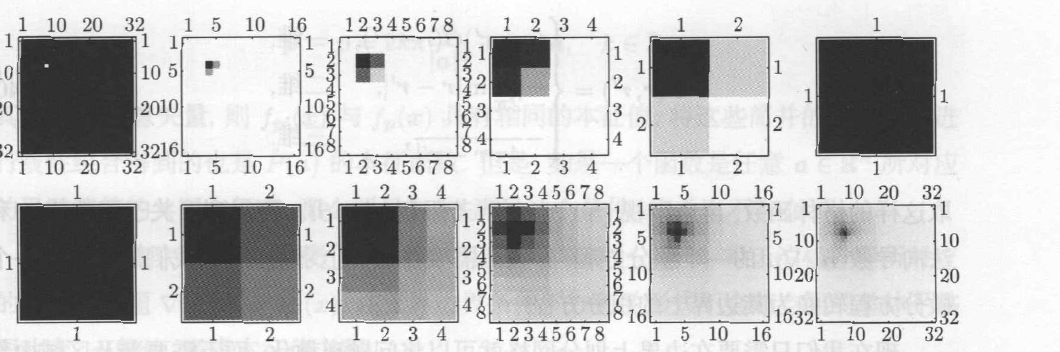
\includegraphics[width=0.96\linewidth]{figures/fig5_2_multigrid.png}
\caption{$32\times32$ 网格下，使用多重网格法求解 $f(x,y)=\delta(x-1/4)\delta(y-1/4)$ 泊松方程的迭代过程}
\label{fig:multigrid-process}
\end{figure}

利用系统在尺度变换下的相似性来求解系统的行为，这个思想在其他物理问题上也获得了广泛应用，一个著名的例子就是统计物理中的重整化群方法。

\subsection{边界元法}

如果问题的求解域不是四四方方那么规则，例如静电学中各种形状的电容器，如何划分网格便成了一个重要问题。边界元法能够部分解决这个困难。我们回顾一下关于格林函数的理论。依旧以泊松方程为例，对于 $\bm r\in\Omega$ 上的微分方程
\begin{equation}
-\nabla_{\bm r}^2u(\bm r)=f(\bm r),
\tag{5.1.37}
\end{equation}
其格林函数定义为如下方程的解：
\begin{equation}
-\nabla_{\bm r}^2G(\bm r,\bm r')=\delta(\bm r-\bm r').
\tag{5.1.38}
\end{equation}
使用数学物理方法中常用的技巧：两式相乘相减积分，并运用格林公式，有
\begin{align}
u(\bm r')&=\int_\Omega G(\bm r,\bm r')f(\bm r)\,\mathrm d^n r\notag\\
&\quad+\int_{\partial\Omega}\left[G(\bm r,\bm r')\nabla_{\bm r}u(\bm r)-u(\bm r)\nabla_{\bm r}G(\bm r,\bm r')\right]\cdot\mathrm d\bm\Sigma.
\tag{5.1.39}
\end{align}
如果 $G(\bm r,\bm r')$ 满足相应的齐次边界条件（例如，边界条件由 $u$ 在 $\partial\Omega$ 上的值给出，则要求 $G(\bm r,\bm r')=0,\ \forall\bm r\in\partial\Omega$），那么问题便得到简化。\footnote{本节没有必要展开讨论如何数值求解偏微分方程的全部细节。}

一般问题的格林函数并没有那么好求解，但是如果不限制边界条件的话，格林函数是不难得到的。对于泊松方程，自由空间中不同维度下满足 (5.1.38) 的格林函数可取为
\begin{equation}
G(\bm r,\bm r')=
\begin{cases}
-\dfrac12|r-r'|,&\text{一维},\\[5pt]
-\dfrac1{2\pi}\ln|\bm r-\bm r'|,&\text{二维},\\[7pt]
\dfrac1{4\pi|\bm r-\bm r'|},&\text{三维}.
\end{cases}
\tag{5.1.40}
\end{equation}
\jiaokan{原印本式 (5.1.40) 的一维项写为 $(r-r')\Theta(r-r')$，三维项写为 $-1/(4\pi|\bm r-\bm r'|)$。它们与紧接在前的定义 $-\nabla^2G=\delta$ 的符号不一致。这里改为标准基本解：一维 $-|r-r'|/2$（与其他一维基本解可相差齐次线性函数），二维 $-(2\pi)^{-1}\ln|\bm r-\bm r'|$，三维 $(4\pi|\bm r-\bm r'|)^{-1}$。}
取这样的格林函数，再来审视 (5.1.39) 式。若限制 $\bm r'\in\partial\Omega$，便得到了关于函数值 $u$ 和法向导数 $\bm n\cdot\nabla u$ 的一个积分方程，并且只需要在边界上求解——我们成功地将一个微分方程转换为其边界上的积分方程！

现在我们只需要在边界上划分网格就可以将问题离散化，而不需要涉及区域内部的事情了。将积分离散化为某种求和，并联立边界条件，便可以求解一个稠密的线性方程组来获得问题的解。降低维度的代价是让稀疏矩阵变得稠密：由于维度降低一维，所以前面的一维泊松方程问题变成了多维，可以解析计算；格林函数在 $\bm r\to\bm r'$ 处总存在奇异性，尤其是边界上的不光滑点，需要小心处理。求得边界上的值后，可以使用同一个公式求得内部任意一点处的值。

除去降低矩阵维度以及便于处理各类边界之外，边界元法还可以用来处理一类特殊问题——变边界问题。考虑一滴水落在低温的金属表面，它将会自下而上逐步凝结。在凝结的过程中，固态区域和液态区域都是在不断变化的，求解域 $\Omega$ 自身也是待求解的对象。如果此时使用基于网格的求解方法，则每一时刻都得基于新的边界重新划分网格，并在不同网格之间相互做插值，而边界元法则省去了这一步骤，大大降低了求解的复杂性。\footnote{关于边界元法的更多细节，可参考 \url{http://www.boundaryelements.com/}。}



\section{动量空间：傅里叶变换}

我们在第三章和第四章的大作业中两次见到了弹簧振子链，它们的本征向量都由三角函数构成，3.2 节中的电路网络以及 5.1 节中的泊松方程也是如此。这源自空间平移不变性。为此，我们定义平移算符 $\hat P(\bm a)$，
\begin{equation}
\hat P(\bm a)u(\bm x)=u(\bm x-\bm a),
\tag{5.2.1}
\end{equation}
将被作用的函数在空间上整体平移 $\bm a$。显然，指数函数 $f_{\bm p}(\bm x)=\exp(i\bm p\cdot\bm x)$ 是平移算符的本征函数：
\begin{equation}
\hat P(\bm a)f_{\bm p}(\bm x)=\exp(-i\bm p\cdot\bm a)f_{\bm p}(\bm x),
\tag{5.2.2}
\end{equation}
本征值为 $\exp(-i\bm p\cdot\bm a)$。不过，平移算符的本征函数是存在简并的。事实上，若有
\[
\bm p'-\bm p=2k\pi\frac{\bm a}{|\bm a|^2}+\bm q,
\qquad k\in\mathbb Z,\quad \bm q\cdot\bm a=0,
\]
其中 $\bm q$ 为任意与 $\bm a$ 正交的矢量，则 $f_{\bm p'}(\bm x)$ 与 $f_{\bm p}(\bm x)$ 具有相同的本征值。将这些简并的本征函数进行线性组合得到的也是 $\hat P(\bm a)$ 的本征函数。但是，如果一个函数是任意 $\bm a\in\mathbb R^n$ 所对应的平移算符的共同本征态，那么便只有 $f_{\bm p}$ 满足这个条件，简并也不存在了。
\jiaokan{原印本将简并条件写为 $\bm p'-\bm p=2k\pi\bm a/|\bm a|^2+\bm q\times\bm a$，随后又声明 $\bm a\in\mathbb R^n$。叉积只在三维（以及某些特殊推广）中有通常意义；一般 $n$ 维条件应写成任意垂直于 $\bm a$ 的分量 $\bm q$，即 $\bm q\cdot\bm a=0$。正文据此改写，而在三维中原式可视为这种垂直分量的一种参数化。}

平移算符除了作用在函数上，也能作用在其他算符上。例如，对于泊松方程所对应的本征值问题 $\nabla^2u(\bm x)=\lambda u(\bm x)$，在无界边界条件下方程的形式不会随空间的整体平移而改变。一般地，考虑本征值方程
\begin{equation}
\hat L u(\bm x)=\lambda u(\bm x).
\tag{5.2.3}
\end{equation}
如果算符 $\hat L$ 在任意空间平移算符 $\hat P(\bm a)$ 下不变，即
\begin{equation}
\hat P(\bm a)\hat L=\hat L\hat P(\bm a),\qquad \forall\bm a\in\mathbb R^n,
\tag{5.2.4}
\end{equation}
作用在 $f_{\bm p}(\bm x)$ 上，则有
\begin{equation}
\hat P(\bm a)\hat Lf_{\bm p}(\bm x)
=\exp(-i\bm p\cdot\bm a)\hat Lf_{\bm p}(\bm x).
\tag{5.2.5}
\end{equation}
这样 $\hat Lf_{\bm p}(\bm x)$ 也是 $\hat P(\bm a)$ 对应于同一个本征值的本征函数。由于这个结果对于任意 $\bm a$ 都成立，根据之前的讨论我们可以断言 $\hat Lf_{\bm p}(\bm x)$ 只可能是 $f_{\bm p}(\bm x)$ 的常数倍，也就是说
\begin{equation}
\hat Lf_{\bm p}(\bm x)=\lambda_{\bm p}f_{\bm p}(\bm x),
\tag{5.2.6}
\end{equation}
即指数函数同样也是算符 $\hat L$ 的本征函数。

这个结论是更为普适的定理——对称性意味着守恒量的一个特例：空间平移不变性意味着动量守恒。

当然，原则上算符 $\hat L$ 中应当包含着边界条件。加上诸如 $u(0)=u(1)=0$ 这样的固定边界条件之后，算符 $\hat L$ 在空间平移下不再是不变的。但是，我们依旧可以用 $\hat P(\bm a)$ 的本征函数做线性组合，以满足这些边界条件。例如，我们注意到，对于方程
\begin{equation}
-\nabla^2u=\lambda u,
\tag{5.2.7}
\end{equation}
在不考虑边界条件的情况下，$e^{ipx}$ 和 $e^{-ipx}$ 对应着同一个本征值 $p^2$，那么我们取
\begin{equation}
u(x)=e^{ipx}-e^{-ipx}=2i\sin(px),
\tag{5.2.8}
\end{equation}
只要令 $p\times1=k\pi,\ k\in\mathbb Z$，这样组合得到的函数便自然满足边界条件。其余类型的边界条件也是类似的。

据此，上一节所讨论的二维泊松方程所对应矩阵的本征值和本征向量分别为
\begin{equation}
\begin{cases}
 u_{mk}(x,y)=2\sin(\pi mx)\sin(\pi ky),\\
 \lambda_{mk}=\pi^2(m^2+k^2),
\end{cases}
\qquad m,k=1,2,\ldots.
\tag{5.2.9}
\end{equation}
此处给出的本征值与上一节中所给出的形式有所不同，这个差异源自用二阶差分替代二阶导数所带来的误差。得知矩阵 $A$ 的全部本征对后，我们相当于完成了对角化
\begin{equation}
A=QDQ^{\mathrm T},
\tag{5.2.10}
\end{equation}
那么方程的解可以写成
\begin{align}
u(x,y)&=QD^{-1}Q^{\mathrm T}f\notag\\
&=\sum_{m,k}q_{mk}\frac1{\lambda_{mk}}q_{mk}^{\mathrm T}f\notag\\
&=\sum_{m,k}u_{mk}(x,y)\frac1{\lambda_{mk}}
\int u_{mk}(x',y')f(x',y')\,\mathrm dx'\,\mathrm dy'.
\tag{5.2.11}
\end{align}
最后一个等号用到了函数间的内积事实上就是相乘积分。现在，我们便得到了方形边界下泊松方程解的一个解析表达式。这种通过求解非齐次偏微分方程所对应的本征值问题来给出原问题的解的办法被称为\textbf{谱方法}（spectral method）。

但是，单单得到一个解析表达式其实意义并不大：为了计算这个式子，我们需要做一个二重无穷级数的求和，而级数中的每一项都是一个二重积分。因此，我们需要使用数值方法近似计算它。以一维为例，首先是积分，我们可以用简单的梯形积分法
\begin{equation}
a_m=\int_0^1\sin(m\pi x)f(x)\,\mathrm dx
\approx\frac1n\sum_{i=1}^{n-1}\sin\!\left(\frac{\pi mi}{n}\right)f\!\left(\frac{i}{n}\right).
\tag{5.2.12}
\end{equation}
然后是无穷求和，我们可以将其截断成一个有限的求和：
\begin{equation}
u\!\left(\frac{i}{n}\right)
=\sum_{m=1}^{\infty}\sin\!\left(\frac{\pi mi}{n}\right)\frac{a_m}{\lambda_m}
\approx\sum_{m=1}^{n-1}\sin\!\left(\frac{\pi mi}{n}\right)\frac{a_m}{\lambda_m}.
\tag{5.2.13}
\end{equation}
很有趣的是，我们发现这两步构成了一对对偶的操作。这也引出了本节的主题：离散傅里叶变换。

\subsection{离散傅里叶变换}

为了让公式简洁，我们不以满足特定边界条件的三角函数作为基底，而是基于指数函数讨论，三角函数可由指数函数通过取实部或虚部得到。考虑变换
\begin{equation}
\tilde a_j=\frac1{\sqrt n}\sum_{k=0}^{n-1}w_n^{jk}a_k,
\tag{5.2.14}
\end{equation}
其中 $w_n=e^{-2\pi i/n}$ 为 $x^n=1$ 在复平面上的 $n$ 次单位根。(5.2.14) 式相当于一个矩阵向量乘法
\begin{equation}
\tilde{\bm a}=F\bm a,
\tag{5.2.15}
\end{equation}
其中傅里叶变换矩阵
\begin{equation}
(F)_{jk}=\frac1{\sqrt n}w_n^{jk}.
\tag{5.2.16}
\end{equation}
矩阵 $F$ 是一个么正矩阵，其共轭转置等于自身的逆，因为
\begin{align}
(FF^\dagger)_{jk}
&=\frac1n\sum_{m=0}^{n-1}w_n^{jm}w_n^{-mk}
=\frac1n\sum_{m=0}^{n-1}w_n^{(j-k)m}\notag\\
&=\begin{cases}
1,&j=k,\\[3pt]
\dfrac1n\dfrac{1-w_n^{n(j-k)}}{1-w_n^{j-k}},&j\ne k,
\end{cases}\notag\\
&=\delta_{jk}=(I)_{jk}.
\tag{5.2.17}
\end{align}
这意味着我们可以轻松写出逆变换：
\begin{equation}
\bm a=F^\dagger\tilde{\bm a},\qquad
a_k=\frac1{\sqrt n}\sum_{j=0}^{n-1}w_n^{-jk}\tilde a_j.
\tag{5.2.18}
\end{equation}
我们将 $\tilde{\bm a}=F\bm a$ 称为 $\bm a$ 的\textbf{离散傅里叶变换}（discrete Fourier transformation, DFT）。与连续形式的傅里叶级数和傅里叶变换类似，容易证明如下几个重要定理：
\begin{enumerate}[label=(\arabic*)]
\item \textbf{Parseval 定理：} $|\bm a|^2=|\tilde{\bm a}|^2$。
\item \textbf{位移--相移定理：}若有 $b_k=a_{(k+m)\bmod n}$，则 $\tilde b_j=w_n^{-jm}\tilde a_j$；而若 $b_k=w_n^{km}a_k$，则 $\tilde b_j=\tilde a_{(j+m)\bmod n}$。
\item \textbf{卷积定理：}
\end{enumerate}
\begin{equation}
\sum_{k=0}^{n-1}a_k b_{(m-k)\bmod n}
=\sum_{j=0}^{n-1}\tilde a_j\tilde b_j w_n^{-jm}.
\tag{5.2.19}
\end{equation}

\subsection{尺度与分辨率}

离散傅里叶变换是由一个 $n$ 维向量到另一个 $n$ 维向量的变换，这显得有些抽象。我们可以尝试将离散变换重新写成连续变换的形式：
\begin{equation}
\begin{cases}
\displaystyle
\tilde f\!\left(\frac{2\pi j}{L}\right)
=\frac1{\sqrt n}\sum_{i=0}^{n-1}f\!\left(\frac{iL}{n}\right)
\exp\!\left[-i\frac{2\pi j}{L}\times\frac{iL}{n}\right],\\[10pt]
\displaystyle
f\!\left(\frac{iL}{n}\right)
=\frac1{\sqrt n}\sum_{j=0}^{n-1}\tilde f\!\left(\frac{2\pi j}{L}\right)
\exp\!\left[i\frac{2\pi j}{L}\times\frac{iL}{n}\right].
\end{cases}
\tag{5.2.20}
\end{equation}
在这个表达式中，$\bm a$ 来自函数 $f(x)$ 在区间 $[0,L)$ 上以 $\Delta x=L/n$ 为间隔的采样，而得到的 $\tilde{\bm a}$ 被诠释为函数 $\tilde f(k)$ 在区间 $[0,2n\pi/L)$ 上以 $\Delta k=2\pi/L$ 为间隔的采样。通常，我们称 $f(x)$ 为时域上的分布或实空间上的函数，而称 $\tilde f(k)$ 为频域上的分布或动量空间上的函数。上式同时也假定了函数的周期性：
\begin{equation}
f(x+T_x)=f(x),\qquad \tilde f(k+T_k)=\tilde f(k),
\tag{5.2.21}
\end{equation}
其中 $T_x=L,\ T_k=2n\pi/L$。

我们容易发现关系
\begin{equation}
T_x\Delta k=2\pi,\qquad T_k\Delta x=2\pi,
\tag{5.2.22}
\end{equation}
即时域的区间大小决定了频域的分辨率，而时域的分辨率又决定了频域的区间大小。这个关系的后一部分被称为 Nyquist 采样定理，指出为了提取出信号中的高频率分量，时域中采样点的间隔必须小于一定值。这是信号处理中的一个重要定理。

不过，对于希望求解偏微分方程来获知场的行为而言，这个关系给予我们的提示是：为了描述实空间中一个快速振荡的函数，动量空间需要足够大；为了描述分布在实空间中很大一个范围中的函数，动量空间中的格点需要足够密。这样，我们便可以在正式求解方程之前大致估计怎么划分格点才能够保证收敛。

将向量视作函数的采样后，也可以讨论函数的导数了。由
\begin{equation}
f(x)=\frac1{\sqrt n}\sum_{j=0}^{n-1}\tilde f(k_j)\exp(ik_jx),
\tag{5.2.23}
\end{equation}
等式两端对 $x$ 求 $m$ 阶导数，可知
\begin{equation}
f^{(m)}(x)=\frac1{\sqrt n}\sum_{j=0}^{n-1}\tilde f(k_j)(ik_j)^m\exp(ik_jx).
\tag{5.2.24}
\end{equation}
这样，函数导数的傅里叶变换等于函数的傅里叶变换再乘上一些常数。不过，(5.2.24) 式实际上存在着一些微妙的地方。我们做离散傅里叶变换时，动量的取值范围限制在 $[0,T_k)$ 中。这其实具有一定的任意性，由位移--相移定理，我们完全可以选取任意一段长度为 $T_k$ 的区间 $[m\Delta k,T_k+m\Delta k)$ 来描述函数。但是，当我们试图计算导函数时，(5.2.24) 式却会对不同区间给出不同的结果。这个矛盾来源于离散傅里叶变换仅要求函数值在采样点 $\{x_i\}$ 处符合要求，而不管其他位置怎么样。但是函数的导数却完全由 $x_i$ 邻域的行为给出。为了避免这个问题，人们通常约定取对称区间 $[-T_k/2,T_k/2)$。

\subsection{快速傅里叶变换}

离散傅里叶变换为满矩阵与向量的乘法，直接计算的复杂度为 $O(n^2)$。然而，$F$ 的矩阵元极具特殊性，让人不禁思考这个计算过程能否简化。我们来重新审视傅里叶变换
\begin{equation}
\tilde a_j=\frac1{\sqrt n}\sum_{k=0}^{n-1}w_n^{jk}a_k.
\tag{5.2.25}
\end{equation}
为方便起见，假设 $n=2^p$，再将奇数和偶数指标拆分：
\begin{align}
\tilde a_j
&=\frac1{2^{p/2}}\sum_{k=0}^{2^p-1}w_{2^p}^{jk}a_k\notag\\
&=\frac1{2^{p/2}}\left(
\sum_{k=0}^{2^{p-1}-1}w_{2^{p-1}}^{jk}a_{2k}
+w_{2^p}^{j}\sum_{k=0}^{2^{p-1}-1}w_{2^{p-1}}^{jk}a_{2k+1}
\right)\notag\\
&=\frac1{\sqrt2}\left(\tilde b_j+w_{2^p}^{j}\tilde c_j\right),
\tag{5.2.26}
\end{align}
其中 $\tilde{\bm b}$ 和 $\tilde{\bm c}$ 分别为 $b_k=a_{2k}$ 和 $c_k=a_{2k+1}$ 的傅里叶变换。这里使用了傅里叶变换的周期性 $\tilde b_{j+2^{p-1}}=\tilde b_j,\ \tilde c_{j+2^{p-1}}=\tilde c_j$。我们发现了一个有趣的结果：一个 $2^p$ 维向量的傅里叶变换，能够写成两个 $2^{p-1}$ 维向量的傅里叶变换的线性组合。显然，我们可以重复地拆分下去，设 $2^p$ 维离散傅里叶变换的计算消耗为 $f(2^p)$，那么有
\begin{equation}
f(2^p)=2f(2^{p-1})+O(2^p).
\tag{5.2.27}
\end{equation}
这个迭代式可以使用常数变易法求解，结果为
\begin{equation}
f(2^p)=O(p2^p).
\tag{5.2.28}
\end{equation}
若用矩阵维度 $n$ 表示，那么如此计算傅里叶变换的计算复杂度为 $O(n\log n)<O(n^2)$。这便是著名的\textbf{快速傅里叶变换}（fast Fourier transform, FFT），伪代码如下。

\begin{algorithmBox}[算法 5.2\quad 快速傅里叶变换]
\begin{lstlisting}[style=bellacode]
function FFT(a,p)
  if(p=0)
    fa = a
  else
    n = 2^(p-1)
    do j = 0,n-1
      b(j) = a(2*j)
      c(j) = a(2*j+1)
    end
    fb = FFT(b,p-1)
    fc = FFT(c,p-1)
    do j = 0,n-1
      fa(j)   = (fb(j) + fc(j)*exp(-pi*I*j/n))/sqrt(2)
      fa(j+n) = (fb(j) - fc(j)*exp(-pi*I*j/n))/sqrt(2)
    end
  end
  return fa
end
\end{lstlisting}
\end{algorithmBox}

历史上，Gauß 最早在其生前未发表的手稿中给出了类似的算法。而其在现代计算机上的广泛应用则要归功于 Cooley 和 Tukey 在 1965 年的重新发现。关于其中的历史，感兴趣的读者可以参考相关文献\footnote{Heideman M T, Johnson D H, and Burrus C S. ``Gauss and the history of the fast Fourier transform.'' \textit{IEEE ASSP Magazine}, 1984, 1(4): 14.}。

上文所给出的快速傅里叶变换要求向量维度 $n$ 是 2 的整数次。事实上，(5.2.26) 式的思想可以用于任意因子的分解。考虑 $n$ 的因数分解
\begin{equation}
n=p_1p_2\cdots p_m,
\tag{5.2.29}
\end{equation}
那么对于任意整数 $k\in[0,n)$，可以做分解 $k=p_1q+r$。我们能将 $n$ 维离散傅里叶变换拆成 $p_1$ 个 $n/p_1$ 维离散傅里叶变换的组合：
\begin{align}
\tilde a_j
&=\frac1{\sqrt n}\sum_{k=0}^{n-1}w_n^{jk}a_k\notag\\
&=\frac1{\sqrt n}\sum_{r=0}^{p_1-1}w_n^{jr}
\sum_{q=0}^{n/p_1-1}w_{n/p_1}^{jq}a_{p_1q+r}\notag\\
&=\frac1{\sqrt{p_1}}\sum_{r=0}^{p_1-1}w_n^{jr}\tilde b_r.
\tag{5.2.30}
\end{align}
那么，计算 $n$ 维离散傅里叶变换的计算消耗 $f(n)$ 为
\begin{align}
f(n)
&=p_1f(n/p_1)+np_1\notag\\
&=p_1p_2f(n/p_1p_2)+np_2+np_1\notag\\
&=\cdots\notag\\
&=n[p_1+p_2+\cdots+p_m+O(1)],
\tag{5.2.31}
\end{align}
即 $n$ 的全部因子之和与 $n$ 的乘积。注意到
\begin{equation}
pq=(p/2-1)q+p(q/2-1)+p+q\ge p+q,
\tag{5.2.32}
\end{equation}
不等号当 $p,q\ge2$ 时成立，那么可以得知，最优的分解方案为将 $n$ 做质因数分解。据此还可以考察一个更有趣的问题：如果我们不再限制 $p_i$ 是整数，而仅要求它们满足 (5.2.29) 式，那么它们取多少时 $f(n)$ 最小？

这是一个约束极值问题，通过 Lagrange 乘子法容易检验取极值时全部 $p_i$ 相等，记作 $p$。那么此时有 $k=\log_p n$，进而
\begin{equation}
f(n;p)=\frac{p}{\ln p}\,n\ln n.
\tag{5.2.33}
\end{equation}
问题进一步约化成了函数 $p/\ln p$ 的极小值问题。令其导数为零，容易得到 $p=e\approx2.718$，为自然对数的底。

我们当然不可能用 $e$ 来做分解。在实际计算中，应该选择 $p=2$ 或 $3$。严格来说，对于差不多大小的 $n$，我们取其为 3 的整数次做快速傅里叶变换要比取 2 的整数次来得更快。

事实上，完全相同的数表达式也出现在了计算机最底层的设计上：用几进制来存储数据最节省资源？答案是三进制。然而如今却是二进制计算机大行其道，这源于在物理上实现二进制要比三进制容易得多，而它们两者之间效率的差距并不是太大：
\begin{equation}
2/\ln2\approx2.885,\qquad 3/\ln3\approx2.730,
\tag{5.2.34}
\end{equation}
不足以抵消物理实现难易度上的巨大差异。同样地，在快速傅里叶变换这个问题上，由于在二进制计算机上做与 2 相关的存储和运算更快，人们也一般以 2 的整数次取格点来划分网格，然后用以执行快速傅里叶变换。

有些情况下，格点数目 $n$ 无法人为控制，实践上也可以考虑手动增加向量的维度以凑 $2^p$，并且令那些多出来的分量为零。需要注意的是，这种处理可能会引入额外的干扰信号，请读者小心。

下一个问题是将算法扩展到多维。对于二维傅里叶变换
\begin{equation}
\tilde a_{ij}=\frac1n\sum_{k,l}a_{kl}w_n^{ik}w_n^{jl},
\tag{5.2.35}
\end{equation}
\jiaokan{原印本式 (5.2.35) 漏写了归一化因子。依本节一维变换的约定，每个维度的 DFT 都带 $1/\sqrt n$，故二维变换应带总因子 $1/n$。若沿用原式，则与 (5.2.14)--(5.2.18) 的么正归一化不一致。}
我们可以先对于求和式中的每一个给定的 $k$，都执行一次快速傅里叶变换，将指标 $l$ 变成 $j$，时间消耗为 $O(n\times n\log n)$，然后再对于每一个给定的 $j$，同样执行一次快速傅里叶变换，将指标 $k$ 变成 $i$。这样，我们便以 $O(2n^2\log n)$ 的时间消耗完成了二维傅里叶变换。容易检验，对于 $d$ 维的情形，快速傅里叶变换的时间消耗为 $O(dn^d\log n)$。

拥有了快速傅里叶变换后，解析式 (5.2.11) 的计算消耗便从直接求解的 $O(n^4)$ 降低为 $O(n^2\log n)$。我们在表 5.1 中列出 $d$ 维空间中泊松方程在每个维度上格点均为 $n$ 时，各个算法的计算消耗。

\begin{table}[htbp]
\centering
\caption{各个算法的计算消耗}
\begin{tabular}{@{}lc@{}}
\toprule
算法 & 计算消耗\\
\midrule
Gauß 消元 & $O(n^{3d})$\\
带状矩阵 Gauß 消元 & $O(n^{3d-2})$\\
Jacobi 迭代/Gauß--Seidel 迭代/最速下降 & $O(n^{d+2})$\\
共轭梯度 & $O(n^{d+1})$\\
快速傅里叶变换 & $O(n^d\log n)$\\
多重网格 & $O(n^d)$\\
\bottomrule
\end{tabular}
\label{tab:complexity-poisson}
\end{table}

\subsection{快速傅里叶变换的其他应用}

除了用于求解偏微分方程外，快速傅里叶变换也能用于加速许多计算。例如，两个向量的卷积（等式左边需要计算 $0\le m\le n-1$ 的全部值）
\begin{equation}
\sum_{k=0}^{n-1}a_kb_{(m-k)\bmod n}
=\sum_{j=0}^{n-1}\tilde a_j\tilde b_jw_n^{-jm},
\tag{5.2.36}
\end{equation}
直接计算的时间复杂度为 $O(n^2)$，但是由卷积定理，可以拆成三个傅里叶变换，那么时间消耗便降低至 $O(n\log n)$。

卷积运算的一个来源是多项式乘法。考虑 $f(x)=\sum_i a_ix^i$ 与 $g(x)=\sum_i b_ix^i$，其乘积为
\begin{equation}
f(x)g(x)=\sum_k x^k\sum_{i=0}^k a_i b_{k-i},
\tag{5.2.37}
\end{equation}
即两个多项式乘积的系数为子多项式系数的卷积。

% R15 extends through source PDF scan p.199 / printed p.184, completing Section 5.2.

\originalpage{200}{185}
另一个来源是 $n\times n$ 维循环矩阵 $(A)_{i,j}=(a)_{(i-j)\bmod n}$ 的线性代数方程组
\begin{equation}
A\bm x=\bm b,
\qquad
\sum_{j=0}^{n-1}a_{(i-j)\bmod n}x_j=b_i.
\tag{5.2.38}
\end{equation}
可以对等式两端同时做傅里叶变换，再借助卷积定理得到
\begin{equation}
\sqrt n\,\tilde a_i\tilde x_i=\tilde b_i.
\tag{5.2.39}
\end{equation}
方程变成了对角的形式。同样三次快速傅里叶变换便能求解，时间消耗为 $O(n\log n)$。循环矩阵的本征值问题也是类似的。

此外，快速傅里叶变换在数论和大整数乘法中也有一些应用。由于其偏离了本书的主旨，这里不再阐述。

\section{分离变量：本征值问题与 Sturm--Liouville 型方程}

在上一节中，我们讨论了拉普拉斯算符的平移不变性以及相应的傅里叶变换。通过找寻算符 $\hat L$ 所满足的对称性，我们轻松求解了本征值问题
\begin{equation}
\hat L u_n=\lambda_n u_n,
\tag{5.3.1}
\end{equation}
然后借助求得的本征值和本征函数，很容易地写下最初偏微分方程 $\hat L u=f$ 的解
\begin{equation}
u=\sum_n\frac1{\lambda_n}u_n\times(u_n,f),
\tag{5.3.2}
\end{equation}
其中 $(u_n,f)=\int u_n(x)f(x)\,\mathrm dx$ 是函数 $u_n$ 与 $f$ 之间的内积。

这套思路可以推广到其他的偏微分方程。例如，考虑氢原子系统的含时 Schrödinger 方程
\begin{equation}
\left(i\partial_t+\frac12\nabla^2+\frac1r\right)\Psi(\bm r,t)=0.
\tag{5.3.3}
\end{equation}
首先，系统具有时间平移不变性，那么算符 $i\partial_t-H$ 的本征函数一定也是时间平移算符的本征函数
\begin{equation}
\psi(\bm r)e^{-iEt}.
\tag{5.3.4}
\end{equation}
将上式代入 (5.3.3) 式中，有
\begin{equation}
\left(-\frac12\nabla^2-\frac1r\right)\psi(\bm r)=E\psi(\bm r).
\tag{5.3.5}
\end{equation}

\originalpage{201}{186}
一个四维的问题约化成了一个三维的本征值问题，我们可以进一步约化。注意到系统在绕坐标原点的任意旋转操作下不变，那么这个三维问题的解也一定是转动算符的本征函数\footnote{转动算符的本征值是简并的，这会使情况稍微有些复杂。}：
\begin{equation}
R_l(r)Y_{lm}(\theta,\phi),
\tag{5.3.6}
\end{equation}
这里 $Y_{lm}(\theta,\phi)$ 是球谐函数。再将 (5.3.6) 式代入 (5.3.5) 式中，有
\begin{equation}
\left[-\frac1{2r^2}\frac{\mathrm d}{\mathrm dr}r^2\frac{\mathrm d}{\mathrm dr}
+\frac{l(l+1)}{2r^2}-\frac1r\right]R_l(r)=ER_l(r),
\tag{5.3.7}
\end{equation}
约化成了一个一维的本征值问题。当然，我们知道对于 Coulomb 势而言，还存在一个额外的动力学对称性，这让上式的解也可以写成一个对称操作的本征函数\footnote{可以参考曾谨言的《量子力学》第二卷第八章的相关内容。}。不过这就略微有些跑题了。这套操作在一般的教材中通常以分离变量法的形式给出，而在此我们需要强调的是，分离变量之所以可行，就是因为系统存在着相应的对称性。

我们在本节中关注的核心问题是：通过一系列变量分离操作后，能得到一个或者数个难以解析求解的一维本征值问题，那么该如何在数值上求解？

\subsection{Sturm--Liouville 型方程}

一般地，我们假设最后得到的一维本征值问题具有下述形式：
\begin{equation}
\left\{
\begin{aligned}
-[p(x)u']'+q(x)u&=\lambda w(x)u,\\
\left.(u\cos\alpha-p(x)u'\sin\alpha)\right|_{x=a}&=0,\\
\left.(u\cos\beta-p(x)u'\sin\beta)\right|_{x=b}&=0,
\end{aligned}\right.
\tag{5.3.8}
\end{equation}
在 $(a,b)$ 上有 $p(x)>0,w(x)>0$。这类问题被称为 Sturm--Liouville（SL）型方程。

这个方程相当于一个实对称矩阵的广义本征值问题
\begin{equation}
\hat L u=\lambda\hat S u,
\tag{5.3.9}
\end{equation}
其中算符 $\hat L=-\dfrac{\mathrm d}{\mathrm dx}\!\left[p(x)\dfrac{\mathrm d}{\mathrm dx}\right]+q(x)$，$\hat S=w(x)$ 都相当于函数空间中的实对称矩阵。我们来证明这一点。

\originalpage{202}{187}
设 $f,g$ 都是满足相应边界条件的平方可积函数，考虑
\begin{align}
(f,\hat Lg)
&=\int_a^b\{-f[p(x)g']'+fq(x)g\}\,\mathrm dx\notag\\
&=\int_a^b\{p(x)f'g'+q(x)fg\}\,\mathrm dx-\left.fp(x)fg'\right|_a^b\notag\\
&=\int_a^b\{-g[p(x)f']'+fq(x)g\}\,\mathrm dx
 +\left.[gp(x)f'-fp(x)g']\right|_a^b\notag\\
&=(g,\hat Lf)+\left.W[f,g](x)\right|_a^b,
\tag{5.3.10}
\end{align}
其中
\begin{equation}
W[f,g](x)\equiv
\begin{vmatrix}
g(x)&f(x)\\
p(x)g'(x)&p(x)f'(x)
\end{vmatrix}
\tag{5.3.11}
\end{equation}
为 Wronski 行列式。由于 $f,pf'$ 和 $g,pg'$ 在边界处满足相同的线性约束，因此该行列式在边界处为零，从而有
\begin{equation}
(f,\hat Lg)=(g,\hat Lf).
\tag{5.3.12}
\end{equation}
“矩阵”是对称的。而对应等式 (5.3.9) 右侧的内积
\begin{equation}
(f,\hat Sg)=\int_a^b f(x)g(x)w(x)\,\mathrm dx,
\tag{5.3.13}
\end{equation}
显然对应一个对称正定矩阵。

若 $f$ 和 $g$ 都是 SL 型方程同一个本征值对应的本征函数，容易检验 Wronski 行列式是一个常量：
\begin{align}
\frac{\mathrm d}{\mathrm dx}W[f,g](x)
&=g'pf'+g(pf')'-f'pg'-f(pg')'\notag\\
&=gw\lambda f-fw\lambda g\notag\\
&=0.
\tag{5.3.14}
\end{align}

在 3.5 节中讨论过，实对称矩阵的本征值问题 $\hat L u=\lambda\hat S u$ 等价于一个二次型的约束极小值问题。或者说，在引入 Lagrange 乘子消去约束后的二次型极小值问题：
\begin{equation}
\min_{u(x),\lambda}\big[(u,\hat L u)-\lambda(u,\hat S u)\big].
\tag{5.3.15}
\end{equation}
将上式具体写开，并且用 $Q(x)$ 替代 $u(x)$，我们可以得到
\begin{equation}
S[Q(x);\lambda]
=\int_a^b[pQ'^2+(q-\lambda w)Q^2] \,\mathrm dx
-\left.pQQ'\right|_a^b.
\tag{5.3.16}
\end{equation}

\originalpage{203}{188}
如果暂时遮去 $\lambda$ 和边界项不管，把 $x$ 看作时间变量，$Q$ 作为广义坐标，关于 $Q(x)$ 的泛函 $S$ 看作某个单自由度系统的作用量，那么被积函数 $pQ'^2+(q-\lambda w)Q^2$ 就成了该系统的 Lagrange 量 $L$，对应有广义动量和 Hamilton 量：
\begin{equation}
\left\{
\begin{aligned}
P&=\frac{\partial L}{\partial Q'}=2pQ',\\
H&=PQ'-L=\frac{P^2}{4p}+(\lambda w-q)Q^2.
\end{aligned}\right.
\tag{5.3.17}
\end{equation}
从而，SL 型方程在一定程度上等价于一个“含时”Hamilton 方程。作为一个最简单的例子，弦上驻波在空间上所满足的方程与一个简谐振子在时间上所满足的方程是一致的。从这个角度来看，Wronski 行列式守恒其实对应着 Hamilton 系统的辛结构守恒。

实对称矩阵的本征值 $\lambda$ 都是实数，且对应于不同本征值的本征函数相互正交：
\begin{equation}
(\lambda_1-\lambda_2)(u_1,\hat S u_2)
=(u_1,\hat L u_2)-(u_2,\hat L u_1)=0.
\tag{5.3.18}
\end{equation}
请注意此处正交指的是 $(u_1,\hat S u_2)=0$，而非通常的 $(u_1,u_2)=0$。

此外，这个系统的本征值
\begin{align}
\lambda
&=\frac{(u,\hat L u)}{(u,\hat S u)}\notag\\
&=\frac{\displaystyle\int_a^b p(x)|u'|^2\,\mathrm dx
+\displaystyle\int_a^b\frac{q(x)}{w(x)}u^2w(x)\,\mathrm dx
-\left.puu'\right|_a^b}
{\displaystyle\int_a^b u^2w(x)\,\mathrm dx}.
\tag{5.3.19}
\end{align}
对于固定边界条件 $\alpha=\beta=0$ 或 $\pi/2$ 的情形，上式大于 $\min_{x\in(a,b)}q(x)/w(x)$，从而存在下界。对于其他情形同样也可以证明本征值存在着类似的下界。因此我们可以由小到大给本征值排序：$\lambda_0<\lambda_1<\lambda_2<\cdots$。另外两条重要性质证明起来比较烦琐，这里直接给出。设 $u_k(x)$ 为 $\lambda_k$ 对应的本征函数，那么有：
\begin{enumerate}[label=(\arabic*)]
\item \textbf{振荡定理：}$u_k(x)$ 在 $(x_1,x_2)$ 上具有 $k$ 个不同零点；$u_k(x)$ 的任意两个相邻零点之间有且仅有 $u_{k-1}$ 的一个零点。
\item $\{u_k(x)\}$ 构成 $L_2(a,b)$ 上的一组正交完备基。
\end{enumerate}
求解此类本征值方程原则上来讲不是什么新问题：使用前两节介绍过的方法，可以将微分方程问题离散化为矩阵问题。再借助 3.4 节中的知识，或直接对角化，或迭代求解，可以得到相应矩阵问题所需的本征值和本征向量。两个问题的本征值直接一一对应，而本征向量和本征函数之间也可以简单转换。然而，根据本征函数的振荡定理，我们的离散化方法往往只能较好地描述前数个本征函数，因为较大的本征值对应于高频的振荡行为，从而难以精确求解。

\originalpage{204}{189}
\subsection{打靶法}

在讨论矩阵化之前，我们先考察一下在 5.1 节中讨论过的边值问题的打靶法。它也可以用于求解本征值问题，但需要做一些修正。

我们知道 $u(x)=0$ 是满足微分方程以及相应的边界条件的，但是显然这不是我们需要的解。若任意取一个 $\lambda$ 值，使用原始形式的打靶法求解，除非我们正好选中了本征值，否则得到的一定是零解！这是由线性齐次方程的特性决定的。

具体来说，当我们选取一端的初值为
\[
u(a)=\gamma\sin\alpha,\qquad pu'(a)=\gamma\cos\alpha
\]
后，为使另一端的残差
\[
\delta(\gamma,\lambda)=u(b)\cos\beta-pu'(b)\sin\beta=\gamma\Delta(\lambda)
\]
为零，需要调整的不是这一端的 $\gamma$，而是本征值 $\lambda$。此时，我们面临的是关于 $\lambda$ 的一个非线性方程的求解问题。

从一头往另一头传播方程可能会引入人为的不稳定性和非对称性。一种解决策略是取一点 $c\in(a,b)$，以某个满足边界条件的初值分别从 $a$ 处和 $b$ 处沿反方向向传播，得到两个函数 $u_1$ 和 $u_2$，再计算它们之间的 Wronski 行列式
\begin{equation}
D(\lambda)=
\begin{vmatrix}
pu_1'(c;\lambda)&pu_2'(c;\lambda)\\
u_1(c;\lambda)&u_2(c;\lambda)
\end{vmatrix}.
\tag{5.3.20}
\end{equation}
如果行列式为零，则两函数线性相关，为该本征值问题的解。从而我们通过求解 $D(\lambda)=0$ 这个关于 $\lambda$ 的非线性方程可得解。

在开头我们讨论了 SL 型方程和 Hamilton 方程的等价性。那么专为 Hamilton 方程设计的辛算法便可以作为打靶法的一种具体实现。

\subsection{Prüfer 变换}

容易看出，本征值问题中存在一个额外的自由度：本征函数乘以任意常数仍然是本征函数。能否将这个自由度消去以简化问题？我们引入 Prüfer 变换\footnote{可注意该方法与量子力学中 WKB 近似的关联。}
\begin{equation}
pu'=r\cos\theta,\qquad u=r\sin\theta.
\tag{5.3.21}
\end{equation}
微分方程和边界条件化为
\begin{equation}
\left\{
\begin{aligned}
(\ln r)'&=(1/p-\lambda w+q)\sin\theta\cos\theta,\\
\theta'&=\cos^2\theta/p+(\lambda w-q)\sin^2\theta,\\
\theta(a)&=\alpha,\\
\theta(b)&=\beta+k\pi.
\end{aligned}\right.
\tag{5.3.22}
\end{equation}

\originalpage{205}{190}
从而方程被拆分成了两个一阶非线性方程，并且其中一个可以单独求解得到本征值——从打靶法的视角来看，这确实降低了求解的复杂度。

我们看到，边界条件中出现了 $k\pi$，这来源于反正切函数，但也可以与本征函数的零点个数相联系\footnote{请思考，如何从这个角度证明振荡定理？请注意 $\theta$ 对 $\lambda$ 的偏导数是恒正的。}。当求解较大的本征值时，方程的条件数会升高，成为刚性问题。这个方程同样可以使用从两头向中间的打靶法。对于某些问题，可以通过恰当地引入一个额外的尺度因子 $S(x)$ 以简化方程，即
\[
pu'=\sqrt S\,r\cos\theta,\qquad
u=\frac{r}{\sqrt S}\sin\theta.
\]

\subsection{Prüfer 方法}

处理复杂的本征值问题的另一个思路是，将问题在局部简化为简单的问题。具体而言，将 $p(x),q(x),w(x)$ 用分段常数函数取代：
\begin{equation}
-[P(x)u']'+Q(x)u=\lambda W(x)u.
\tag{5.3.23}
\end{equation}
在某一段区域 $[y_{j-1},y_j]$ 中，令区间长度为 $h_j$，三个函数的值分别为 $p_j,q_j,w_j$，定义 $k_j=(\lambda w_j-q_j)/p_j$。这样近似后，在 $[y_{j-1},y_j]$ 这段常数区间内方程简化为谐振子方程
\begin{equation}
u''=-k_j u,
\tag{5.3.24}
\end{equation}
其严格解为
\begin{equation}
u(x)=u(y_{j-1})\Psi_j(x-y_{j-1})+(Pu')(y_{j-1})\Phi_j(x-y_{j-1})/p_j,
\tag{5.3.25}
\end{equation}
其中
\begin{equation}
\Psi_j(x)=
\begin{cases}
\cos(\sqrt{k_j}x),&k_j>0,\\
1,&k_j=0,\\
\cosh(\sqrt{-k_j}x),&k_j<0,
\end{cases}
\qquad
\Phi_j(x)=
\begin{cases}
\sin(\sqrt{k_j}x)/\sqrt{k_j},&k_j>0,\\
x,&k_j=0,\\
\sinh(\sqrt{-k_j}x)/\sqrt{-k_j},&k_j<0.
\end{cases}
\tag{5.3.26}
\end{equation}
相邻两个常数区间取连接条件 $u$ 以及 $Pu'$ 连续，得到
\begin{equation}
\binom{u}{Pu'}_j=T_j\binom{u}{Pu'}_{j-1}.
\tag{5.3.27}
\end{equation}

\originalpage{206}{191}
其中转移矩阵
\begin{equation}
T_j=
\begin{pmatrix}
\cos(\sqrt{k_j}h_j)&\dfrac{\sin(\sqrt{k_j}h_j)}{p_j\sqrt{k_j}}\\[7pt]
-p_j\sqrt{k_j}\sin(\sqrt{k_j}h_j)&\cos(\sqrt{k_j}h_j)
\end{pmatrix}.
\tag{5.3.28}
\end{equation}
那么从一端的初始条件出发，可以通过连乘转移矩阵得到另一端与边界条件的差
\begin{equation}
\delta=(\cos\beta\ -\sin\beta)
\prod_jT_j(\lambda)
\binom{\sin\alpha}{\cos\alpha}.
\tag{5.3.29}
\end{equation}
求解 $\delta(\lambda)=0$ 这个关于 $\lambda$ 的非线性方程，就能得到本征值和本征函数。这种方法称为 Prüfer（Pruess）方法，一定程度上讲，其就是打靶法的一个具体实现，其误差正比于 $p,q,w$ 这三个函数的导数与区间长度 $h_j$ 的乘积。但是由于在近似过程中保持了 SL 型方程的形式，因此方程拥有的诸多解析性质，包括 Wronski 行列式的守恒、不同本征解之间的正交性、振荡定理等都能严格成立。

\subsection{奇异边界条件}

让我们回到本节一开头导出的方程 (5.3.7)，写成 SL 型方程的标准形式
\begin{equation}
-[r^2R_l'(r)]'+[l(l+1)-2r]R_l(r)=2Er^2R_l(r),
\tag{5.3.30}
\end{equation}
这里有 $p(r)=r^2,q(r)=l(l+1)-2r,w(r)=2r^2$，而边界点为 $a=0,b=\infty$。由波函数单值、有界且平方可积可以写下边界条件
\begin{equation}
\left\{
\begin{aligned}
\left.r^2R_l'(r)\right|_{r=0}&=0,\\
\left.R_l(r)\right|_{r=\infty}&=0.
\end{aligned}\right.
\tag{5.3.31}
\end{equation}
这个方程的两个端点都会产生麻烦。

首先是右端的无穷远边界，这意味着无穷大的求解域，那该如何划分格点进行传播呢？最简单的策略是取一个足够大的端点 $r_{\max}$，令波函数在这一点近似为零，然后求解本征值问题。当得到的本征值几乎不随 $r_{\max}$ 的增大而变化时，便认为我们已经求得了一个充分好的解。此外，Prüfer 方法可以将最右侧端点 $r_n$ 取作无穷大，但仍然需要找一个充分大的 $r_{n-1}$。

其次是左端的边界点。这个点粗看起来没什么毛病，但如果考虑到在 Prüfer 方法和 Prüfer 变换中都出现了 $1/p$ 的表达式，而 $1/p$ 在 $r=0$ 处发散时，问题就来了。在量子力学课程的学习中，解析分析告诉我们此处 $R(r)\sim r^l$，这意味着所使用的微分方程解法必须有足够高的精度，才能较好地描述这一点的行为。实践中，处理这类奇异边界的思路和 Prüfer 方法类似：取一个小区间 $[0,\Delta r]$，在这个小区间内用解析的手段给

\originalpage{207}{192}
出本征函数的渐近行为以及 $r=\Delta r$ 处的边界条件，然后再以 $\Delta r$ 为数值处理时使用的左端点来求解方程。

\subsection{数值实验}

现在让我们对 (5.3.7) 式来实际试验一下本书中讨论的算法。我们在 $r\in(0,\infty)$ 上划分格点 $\{a,a+h,a+2h,\ldots,b\}$，在最两端的边界用渐近解来消除奇异性。对于 $r\in(0,a)$ 区间段，有 $R(r)\sim r^l$，从而在 $r=a$ 处
\begin{equation}
\left.r^2R_l'(r)\right|_{r=a}=la^{l+1}=laR_l(a),
\tag{5.3.32}
\end{equation}
故可取 $\cot\alpha=la$。对于另一端 $r\in(b,\infty)$，有 $R(r)\sim e^{-\sqrt{-2E}r}/r$，从而在 $r=b$ 处
\begin{equation}
\left.r^2R_l'(r)\right|_{r=b}
=-e^{-\sqrt{-2E}b}-\sqrt{-2E}\,b e^{-\sqrt{-2E}b}
=-(1+\sqrt{-2E}\,b)bR_l(b),
\tag{5.3.33}
\end{equation}
因此可取 $\cot\beta=-(1+\sqrt{-2E}\,b)b$。我们看到此时本征值也出现在了边界条件中，但这并不影响后面的求解。

消去了奇异边界后，我们尝试使用 Prüfer 算法来求解，各函数用相应区间段中点的值来近似。数值参数取 $l=0,h=0.4,a=h/2=0.2,b=4+a=4.2$。求解方程 $\delta(E)=0$ 得到两个根
\begin{equation}
E_1=-0.4856,\qquad E_2=-0.0142.
\tag{5.3.34}
\end{equation}
在量子力学中我们学过，氢原子束缚态的径向波函数是连带 Laguerre 函数，本征值为 $E=-1/2(n+1)^2$。$-0.4856$ 这个根和氢原子 $1s$ 态能量 $-0.5$ 相去不远，然而 $-0.0142$ 却和 $2s$ 态能量 $-0.125$ 完全不是一回事，更别提氢原子原则上有无穷多个束缚态。

我们猜测这个结果源自数值参数不足以收敛。为此，我们缩小 $h$，数值求得的本征值如表 5.2 所示。

\begin{table}[htbp]
\centering
\caption{$b=4.2$ 时不同 $h$ 得到的本征值}
\begin{tabular}{@{}ccccc@{}}
\toprule
$h$&0.4&0.2&0.1&0.05\\
\midrule
$E_1$&-0.4856&-0.4960&-0.4976&-0.4977\\
$E_2$&-0.0142&-0.0084&-0.0058&-0.0047\\
\bottomrule
\end{tabular}
\end{table}
我们看到，随着格点间距的减小，$E_1$ 不断减小并向理论值靠拢（但并没有收敛到 $-0.5$ 的趋势），而 $E_2$ 始终保持着一个很荒唐的值。这说明问题不出在 $h$ 上，而是出在 $b$ 上。我们依旧取 $h=0.4$，然后增大 $b$，结果如表 5.3 所示。

\originalpage{208}{193}
\begin{table}[htbp]
\centering
\caption{$h=0.4$ 时不同 $b$ 得到的本征值}
\begin{tabular}{@{}cccccc@{}}
\toprule
$b$&4.2&8.2&12.2&16.2&20.2\\
\midrule
$E_1$&-0.4856&-0.4873&-0.4873&-0.4873&-0.4873\\
$E_2$&-0.0142&-0.1156&-0.1249&-0.1256&-0.1256\\
$E_3$&&&-0.0290&-0.0487&-0.0542\\
$E_4$&&&&&-0.0106\\
\bottomrule
\end{tabular}
\end{table}
可以发现，尽管使用了一个较大的格点间距，但 $E_2$ 随着 $b$ 的增大快速向理论值靠近。同时，方程还出现了更多的根。看来，为了容纳更多的本征函数，我们需要足够大的空间；而为了准确描述这些本征函数，我们需要足够小的格点间距。这在物理上也是不难理解的：高量子数的 Rydberg 态是要占据很大的空间。

不论如何，这类方案看起来总不够好：使用了这么多格点，也没能给出一个很精确的解。特别地，如果我们希望方程能同时给出精确的基态和高激发态，那么我们同时得有足够大的空间尺度和足够小的格点间距，这对计算量的要求就更高了。5.4 节中将介绍基于正交多项式的处理手段，那时我们能看到这类问题可以轻松处理。

\begin{exerciseBox}[练习 5.2]
试对于 $r=\infty$ 的边界条件，直接取 $R(b)=0$，并采取和正文中类似的数值参数，求解 (5.3.7) 式，比较你的结果。
\end{exerciseBox}

\subsection{依赖于本征值的边界条件}

我们在之前的处理中为了消去边界的奇异性，引入了依赖于本征值的边界条件。其实，这在某些实际的物理问题中也存在。比方说，考虑一个弹簧振子，其中的弹簧不再视作无质量的理想弹簧，而是可以承载波动的弹性体。

如图 5.3 所示，设原位于 $x$ 处的弹簧微元相对平衡位置在 $t$ 时刻移动了 $u(x,t)$，我们可以写下 $u$ 所满足的波动方程：
\begin{equation}
\left\{
\begin{aligned}
\partial_t^2u-\frac{k\ell^2}{m}\partial_x^2u&=0,\\
u|_{x=0}&=0,\\
\left.M\partial_t^2u+\frac{k}{\ell}\partial_xu\right|_{x=\ell}&=0,
\end{aligned}\right.
\tag{5.3.35}
\end{equation}
其中 $k,\ell,m$ 分别为弹簧的劲度系数、原长和质量，$M$ 为振子的质量。由于系统具有时间平移不变性，故方程的解可以写成 $f(x)e^{i\omega t}$ 的形式。代回 (5.3.35) 式得到
\begin{equation}
\left\{
\begin{aligned}
-\frac{k\ell^2}{m}f''&=\omega^2f,\\
f|_{x=0}&=0,\\
\left.\frac{k}{M\ell}f'\right|_{x=\ell}&=\omega^2f.
\end{aligned}\right.
\tag{5.3.36}
\end{equation}

\originalpage{209}{194}
将 $\omega^2$ 看作本征值，我们发现，它出现在了边界条件上。

\begin{figure}[htbp]
\centering
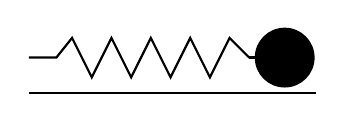
\begin{tikzpicture}[x=1cm,y=1cm,thick]
  \draw (0,0) -- (0.35,0) -- (0.55,0.25) -- (0.8,-0.25) -- (1.05,0.25) -- (1.3,-0.25) -- (1.55,0.25) -- (1.8,-0.25) -- (2.05,0.25) -- (2.3,-0.25) -- (2.55,0.25) -- (2.8,0);
  \fill (3.25,0) circle (0.38);
  \draw (2.8,0) -- (2.87,0);
  \draw (0,-0.45) -- (3.65,-0.45);
\end{tikzpicture}
\caption{有质量的非理想弹簧}
\label{fig:massive-spring}
\end{figure}

\section{变分原理：\rusname{Галёркин}法与函数基组}

前述数节中，我们讨论了如何通过各种各样的方案将微分方程边值问题离散化成线性代数方程组。尽管我们容易分析这些离散方案的局部截断误差，但这些误差对整体结果会产生多大影响，并不存在一般性的理论，5.1 节中对一维泊松方程的分析很难推广到高维度。因此，本节我们将从另一个视角来探讨微分方程的边值问题，这个视角在理论上更为优美，也更容易引出其他更高精度的算法。

在物理上我们知道，常见物理问题的微分方程往往对应着某个泛函 $\int\mathcal L\,\mathrm dV$ 的极值问题，这里 $\mathcal L$ 是 Lagrange 量密度。例如 5.1 节中重点讨论的泊松方程
\begin{equation}
-\nabla^2u=f
\tag{5.4.1}
\end{equation}
对应于
\begin{equation}
\mathcal L=\frac12(\nabla u)^2-uf,
\tag{5.4.2}
\end{equation}
\jiaokan{原印本式 (5.4.2) 写作 $\mathcal L=\tfrac12(\nabla u)^2+uf$。按 Euler--Lagrange 方程变分，原式给出 $-\nabla^2u+f=0$，即 $-\nabla^2u=-f$，与紧邻的 (5.4.1) 符号相反。故将源项改为 $-uf$。}
波动方程
\begin{equation}
(\partial_t^2-\nabla^2)u=0
\tag{5.4.3}
\end{equation}
对应于
\begin{equation}
\mathcal L=(\partial_tu)^2-(\nabla u)^2.
\tag{5.4.4}
\end{equation}
熟知的 Maxwell 方程组
\begin{equation}
\left\{
\begin{aligned}
\nabla\cdot\bm E&=\rho/\epsilon_0,\\
\nabla\times\bm E&=-\partial_t\bm B,\\
\nabla\cdot\bm B&=0,\\
\nabla\times\bm B&=\mu_0\bm J+\mu_0\epsilon_0\partial_t\bm E
\end{aligned}\right.
\tag{5.4.5}
\end{equation}
对应于
\begin{equation}
\mathcal L=\frac{\epsilon_0}{2}(E^2-c^2B^2)-\rho\phi+\bm J\cdot\bm A.
\tag{5.4.6}
\end{equation}
\jiaokan{原印本式 (5.4.6) 的源项写作 $+\rho\phi-\bm J\cdot\bm A$。在通常约定 $\bm E=-\nabla\phi-\partial_t\bm A$、$\bm B=\nabla\times\bm A$ 下，为得到 (5.4.5) 中的 $\nabla\cdot\bm E=\rho/\epsilon_0$ 与 $\nabla\times\bm B=\mu_0\bm J+\mu_0\epsilon_0\partial_t\bm E$，源耦合应为 $-\rho\phi+\bm J\cdot\bm A$，故据此改正。}

% R16 extends through source PDF scan p.209 / printed p.194, completing Section 5.3 and opening Section 5.4.

\originalpage{210}{195}
就连带着复数项的 Schrödinger 方程
\begin{equation}
i\partial_t\Psi=-\frac12\nabla^2\Psi+V\Psi
\tag{5.4.7}
\end{equation}
也能找到相应的 Lagrange 量密度
\begin{equation}
\mathcal L=\frac{i}{2}\left(\Psi^*\partial_t\Psi-\Psi\partial_t\Psi^*\right)-\frac12|\nabla\Psi|^2-V|\Psi|^2.
\tag{5.4.8}
\end{equation}
在量子场论中，Lagrange 量更是超越了运动方程，成为描述物理系统行为最基本的函数，由之可以导出运动方程。

既然是极值问题，我们就可以用极值问题的思路来处理。我们知道，满足给定边界条件的全体平方可积函数构成了一个无穷维线性空间 $L^2$，其中每个函数都可以看作一个向量，诸如梯度、Laplacian 算符之类的算符将一个函数线性地映射到另一个函数，从而可以看作一个矩阵。更进一步，我们看到前面所讨论的 Lagrange 量都是函数的二次型\footnote{当然，实践中也存在很多更复杂的问题。}，也就是说，我们需要在无穷维函数空间中求解如下二次型的极值问题：
\begin{equation}
L=\frac12\bm x^{\mathrm T}A\bm x-\bm x^{\mathrm T}\bm b.
\tag{5.4.9}
\end{equation}
这里的待求向量 $\bm x$ 对应着待求的物理场 $u,(E,B)$ 或 $\Psi$，已知向量 $\bm b$ 对应着源和汇 $f,(\rho,J)$，矩阵 $A$ 则对应着 $-\nabla^2,\partial_t^2-\nabla^2$ 等等这些算符。

无穷维的问题在计算实践中无法处理，我们必须截断为有限维。假设我们选定一组线性无关（未必正交）的函数 $\{e_1,e_2,\ldots,e_n\}$，张成了一个 $n$ 维子空间，那便可以先在这个子空间
\begin{equation}
\bm x=\sum_i e_i c_i=E\bm c
\tag{5.4.10}
\end{equation}
内求 $L$ 的极小值
\begin{equation}
L=\frac12\bm c^{\mathrm T}E^{\mathrm T}AE\bm c-\bm c^{\mathrm T}E^{\mathrm T}\bm b.
\tag{5.4.11}
\end{equation}
这个关于 $n$ 维向量 $\bm c$ 的二次型的极值问题对应于线性代数方程组
\begin{equation}
E^{\mathrm T}AE\bm c=E^{\mathrm T}\bm b,
\tag{5.4.12}
\end{equation}
系数由下式给出：
\begin{equation}
\begin{aligned}
(E^{\mathrm T}AE)_{ij}&=e_i^{\mathrm T}Ae_j=\int e_i(\bm r)\,A e_j(\bm r)\,\mathrm dV,\\
(E^{\mathrm T}\bm b)_i&=e_i^{\mathrm T}\bm b=\int e_i(\bm r)b(\bm r)\,\mathrm dV.
\end{aligned}
\tag{5.4.13}
\end{equation}

\originalpage{211}{196}
完成系数计算和线性方程组求解，我们便给出了原问题的一个近似解。这个解在我们所限定的子空间内是最优的。

此外，我们也可以将 (5.4.12) 式改写成
\begin{equation}
E^{\mathrm T}(AE\bm c-\bm b)=0,
\tag{5.4.14}
\end{equation}
也就是说，通过这种方案得到的近似解，其残差与所选取的子空间正交。那么这种方案到底有多好，就完全依赖于子空间怎么选取。本节将会介绍若干种常见的方案。这类方案被称为\rusname{Галёркин}法。

类似的思路也可以应用于本征值问题之上。从 3.5 节中我们知道，本征值问题 $A\bm x=\lambda\bm x$ 可以转换成一个带 Lagrange 乘子的二次型极值问题
\begin{equation}
L=\bm x^{\mathrm T}A\bm x-\lambda(\bm x^{\mathrm T}\bm x-1).
\tag{5.4.15}
\end{equation}
我们在基组 $\{e_1,e_2,\ldots,e_n\}$ 张成的子空间中求解这个极值问题的解，那么
\begin{equation}
L=\bm c^{\mathrm T}E^{\mathrm T}AE\bm c-\lambda(\bm c^{\mathrm T}E^{\mathrm T}E\bm c-1).
\tag{5.4.16}
\end{equation}
它对应于一个有限维的广义本征值问题
\begin{equation}
E^{\mathrm T}AE\bm c=\lambda E^{\mathrm T}E\bm c,
\tag{5.4.17}
\end{equation}
交叠矩阵由下式给出：
\begin{equation}
(E^{\mathrm T}E)_{ij}=e_i^{\mathrm T}e_j=\int e_i(\bm r)e_j(\bm r)\,\mathrm dV.
\tag{5.4.18}
\end{equation}

\subsection{有限元法}

最简单的基函数是分段线性函数。在区间 $[a,b]$ 中作分划点 $\{x_j\}:a=x_0<x_1<\cdots<x_{n-1}<x_n=b$，取如下形式的基函数：
\begin{equation}
e_j(x)=
\begin{cases}
\dfrac{x-x_{j-1}}{x_j-x_{j-1}},&x_{j-1}<x\le x_j,\\[6pt]
\dfrac{x-x_{j+1}}{x_j-x_{j+1}},&x_j<x\le x_{j+1},\\[6pt]
0,&\text{其他情况}.
\end{cases}
\tag{5.4.19}
\end{equation}
注意这类基函数函数值处处连续，其一阶导数容易计算：
\begin{equation}
e_j'(x)=
\begin{cases}
\dfrac1{x_j-x_{j-1}},&x_{j-1}<x<x_j,\\[6pt]
\dfrac1{x_j-x_{j+1}},&x_j<x<x_{j+1},\\[6pt]
0,&\text{其他情况}.
\end{cases}
\tag{5.4.20}
\end{equation}

\originalpage{212}{197}
导数值在各分划点处存在间断。

此类函数仅在有限区间上非零的特性使得各算符矩阵元非常容易计算，交叠矩阵为
\begin{equation}
e_i^{\mathrm T}e_j=
\frac{x_{i+1}-x_i}{6}\delta_{i,j-1}
+\frac{x_{i+1}-x_{i-1}}{3}\delta_{ij}
+\frac{x_i-x_{i-1}}{6}\delta_{i,j+1}.
\tag{5.4.21}
\end{equation}
导数算符为
\begin{equation}
\left(\frac{\mathrm d}{\mathrm dx}\right)_{ij}
=\int_a^b e_i(x)\frac{\mathrm d}{\mathrm dx}e_j(x)\,\mathrm dx
=\frac{\delta_{i,j-1}-\delta_{i,j+1}}{2}.
\tag{5.4.22}
\end{equation}
二阶导数算符为
\begin{equation}
\begin{aligned}
\left(\frac{\mathrm d^2}{\mathrm dx^2}\right)_{ij}
&=\int_a^b e_i(x)\frac{\mathrm d^2}{\mathrm dx^2}e_j(x)\,\mathrm dx\\
&=\left.e_i(x)e_j'(x)\right|_a^b-\int_a^b e_i'(x)e_j'(x)\,\mathrm dx\\
&=\frac{\delta_{i,j-1}-\delta_{ij}}{x_{i+1}-x_i}
+\frac{\delta_{i,j+1}-\delta_{ij}}{x_i-x_{i-1}}.
\end{aligned}
\tag{5.4.23}
\end{equation}
注意这里使用了一次分部积分，消去了间断点。其余与坐标直接依赖的算符 $g(x)$ 同样是三对角的：
\begin{equation}
\begin{aligned}
(\hat g)_{ij}&\equiv\int_a^b e_i(x)g(x)e_j(x)\,\mathrm dx\\
&=\delta_{i,j-1}\int_{x_i}^{x_{i+1}}g(x)\frac{(x_{i+1}-x)(x-x_i)}{(x_{i+1}-x_i)^2}\,\mathrm dx\\
&\quad+\delta_{ij}\left[\int_{x_{i-1}}^{x_i}g(x)\left(\frac{x-x_{i-1}}{x_i-x_{i-1}}\right)^2\,\mathrm dx
+\int_{x_i}^{x_{i+1}}g(x)\left(\frac{x_{i+1}-x}{x_{i+1}-x_i}\right)^2\,\mathrm dx\right]\\
&\quad+\delta_{i,j+1}\int_{x_{i-1}}^{x_i}g(x)\frac{(x_i-x)(x-x_{i-1})}{(x_i-x_{i-1})^2}\,\mathrm dx.
\end{aligned}
\tag{5.4.24}
\end{equation}

使用此类分段线性基函数的微分方程解法被称为有限元法 (finite element method)。有限元法很容易推广到高维度。我们以二维为例，假定在求解域 $\Omega$ 上有一系列分划点 $P_l:(x_l,y_l)$。以这些点为顶点，$\Omega$ 被切分成一系列三角形区域\footnote{关于网格的划分算法，可以参考 Edelsbrunner H. \textit{Geometry and Topology for Mesh Generation}. Cambridge University Press, 2001.}。对于每一个顶点 $P_l$，我们构造分段线性基函数 $\varphi_l(x)$，它在不以 $P_l$ 为顶点的三角形内为零，而在此类三角形内非零：
\begin{equation}
\varphi_{l(mn)}(x,y)=
\frac{\begin{vmatrix}x&y&1\\x_n&y_n&1\\x_m&y_m&1\end{vmatrix}}
{\begin{vmatrix}x_l&y_l&1\\x_n&y_n&1\\x_m&y_m&1\end{vmatrix}},
\qquad x\in\Delta_{lmn}.
\tag{5.4.25}
\end{equation}

\originalpage{213}{198}
其中 $\Delta_{lmn}$ 表示以 $P_l,P_n,P_m$ 为顶点构成的三角形。容易检验，这个线性函数等于 $\Delta PP_nP_m$ 与 $\Delta_{lmn}$ 面积之比，如图 5.4 所示。将三角形替换成相应维度下的单纯形，这类行列式的写法也很容易向更高的维度推广。

\begin{figure}[htbp]
\centering
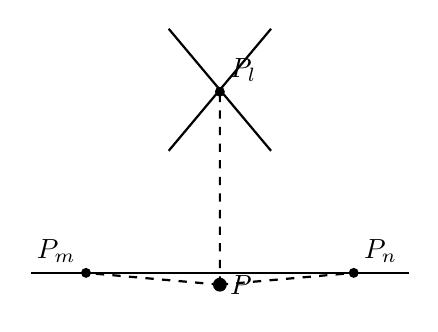
\begin{tikzpicture}[scale=1.0,thick]
  \coordinate (Pl) at (0,2.3);
  \coordinate (Pm) at (-1.7,0);
  \coordinate (Pn) at (1.7,0);
  \coordinate (P) at (0,-0.15);
  \draw (-0.65,3.1)--(0.65,1.55);
  \draw (0.65,3.1)--(-0.65,1.55);
  \draw (-2.4,0)--(2.4,0);
  \draw[dashed] (P)--(Pl) (P)--(Pm) (P)--(Pn);
  \fill (Pl) circle (1.8pt) node[above right]{$P_l$};
  \fill (Pm) circle (1.8pt) node[above left]{$P_m$};
  \fill (Pn) circle (1.8pt) node[above right]{$P_n$};
  \fill (P) circle (2.5pt) node[right]{$P$};
\end{tikzpicture}
\caption{二维三角形区域划分下有限元法基函数示意图}
\label{fig:fe-triangle-basis}
\end{figure}

随后考虑矩阵元。作为示例，这里给出基函数 $\varphi_l$ 和 $\varphi_m$ 之间的 Laplacian 算符 $-\nabla^2$ 在一个三角形 $\Delta_{lmn}$ 内\footnote{注意，二维情况下，基函数 $\varphi_l$ 和 $\varphi_m$ 会在两个不同的三角形中同时非零。}的积分
\begin{equation}
K_{lm(n)}\equiv\int_{\Delta_{lmn}}\nabla\varphi_l\cdot\nabla\varphi_m\,\mathrm dS
=\frac{\overrightarrow{mn}\cdot\overrightarrow{nl}}{S_{\Delta_{lmn}}}.
\tag{5.4.26}
\end{equation}
当迭代求解大规模问题时，由于各种矩阵元的计算都很简单，人们往往会选择用时间换空间，随用随算而不做存储。

有限元法的优势在于灵活方便，对于任意形状的求解区域和各种形式的方程都容易给出一个精度尚可的解，对于弹性体的变形问题也有着不错的适应性。关于它的理论以及商业化程序是非常成熟的，我们不在此做过多介绍。但当对解的精度有更高的要求时，由于其局部截断误差仅为一阶，计算量的增长往往是相当可观的。从而，我们想寻求超越线性的基函数。

\subsection{B 样条插值}

定义
\begin{equation}
B_i^{(0)}(x)=
\begin{cases}
1,&x_i\le x<x_{i+1},\\
0,&\text{其他情况},
\end{cases}
\tag{5.4.27}
\end{equation}
以及 Cox--de Boor 递推公式
\begin{equation}
B_i^{(k)}(x)=\frac{x-x_i}{x_{i+k}-x_i}B_i^{(k-1)}(x)
+\frac{x_{i+k+1}-x}{x_{i+k+1}-x_{i+1}}B_{i+1}^{(k-1)}(x),
\tag{5.4.28}
\end{equation}
我们便给出了 B 样条 (basis spline) 函数的定义。容易看出，$B_i^{(k)}(x)$ 为分段 $k$ 次多项式，在 $[x_i,x_{i+k+1})$ 上恒大于零且小于等于一，而在其余位置为零。

\originalpage{214}{199}
一阶 B 样条函数是分段线性函数，与有限元法所使用的基函数是一致的，在全区间上连续，而二阶 B 样条函数的导数为
\begin{equation}
\begin{aligned}
\frac{\mathrm d}{\mathrm dx}B_i^{(2)}(x)
&=\frac1{x_{i+2}-x_i}B_i^{(1)}(x)
+\frac{x-x_i}{x_{i+2}-x_i}\frac{\mathrm d}{\mathrm dx}B_i^{(1)}(x)\\
&\quad-\frac1{x_{i+3}-x_{i+1}}B_{i+1}^{(1)}(x)
+\frac{x_{i+3}-x}{x_{i+3}-x_{i+1}}\frac{\mathrm d}{\mathrm dx}B_{i+1}^{(1)}(x).
\end{aligned}
\tag{5.4.29}
\end{equation}
我们知道，$B_i^{(1)}(x)$ 在 $x=x_i,x_{i+1},x_{i+2}$ 这三点处导数不连续。然而，上式中的 $x-x_i$ 因子将 $x=x_i$ 处的不连续压低至零，而 $x=x_{i+1}$ 处
\begin{equation}
\begin{aligned}
\lim_{x\to x_{i+1}}\frac{\mathrm d}{\mathrm dx}B_i^{(2)}(x)
&=\frac{x_{i+1}-x_i}{x_{i+2}-x_i}\frac{\mathrm d}{\mathrm dx}B_i^{(1)}(x)
+\frac{x_{i+3}-x_{i+1}}{x_{i+3}-x_{i+1}}\frac{\mathrm d}{\mathrm dx}B_{i+1}^{(1)}(x)+\cdots\\
&=\begin{cases}
\dfrac{x_{i+1}-x_i}{x_{i+2}-x_i}\dfrac1{x_{i+1}-x_i}+\cdots,&x=x_{i+1}-\epsilon,\\[8pt]
\dfrac{x_{i+1}-x_i}{x_{i+2}-x_i}\dfrac{-1}{x_{i+2}-x_{i+1}}+\dfrac1{x_{i+2}-x_{i+1}}+\cdots,&x=x_{i+1}+\epsilon.
\end{cases}
\end{aligned}
\tag{5.4.30}
\end{equation}
式中省略号表示导数表达式中显然连续的部分。我们发现，通过 Cox--de Boor 公式所给出的叠加方案，我们正好将两个导数不连续的函数叠加在一起，使得导数连续了。类似地，容易检验 $B_i^{(2)}(x)$ 在全区间上导数连续。更一般地，我们可以通过数学归纳法证明 $B_i^{(k)}(x)$ 在全区间上 $k-1$ 次连续可微。图 5.5 各子图依此给出了 0 至 3 阶的 B 样条函数。

\begin{figure}[htbp]
\centering
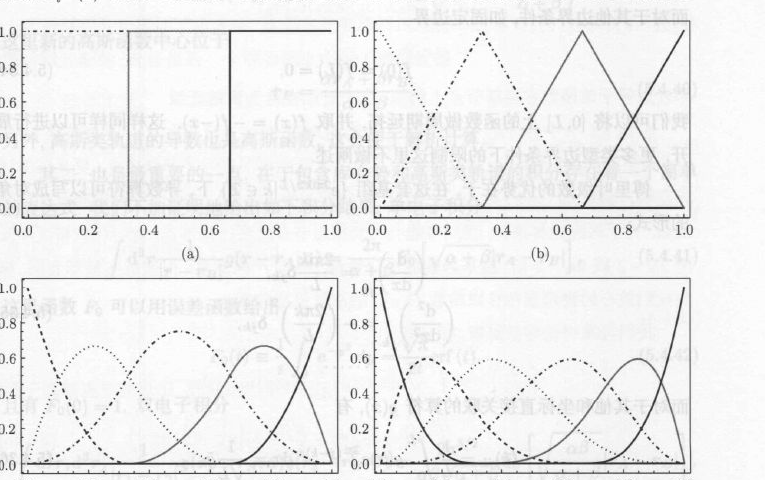
\includegraphics[width=0.92\textwidth]{figures/fig5_5_bspline.png}
\caption{图 (a)、(b)、(c)、(d) 分别表示 0 至 3 阶的 B 样条函数}
\label{fig:bspline-orders}
\end{figure}

\originalpage{215}{200}
样条函数，分点均取作 $(0,0,0,0,1/3,2/3,1,1,1,1)$。

B 样条函数的诸多特性使其在用于数值计算时有不少优势。由于其仅在有限区域中非零，这使得微分方程矩阵化后为带状矩阵，方便求解；分段多项式使得不少矩阵元可以解析计算；高次连续可微使得充分光滑。另外，它并不禁止两个相邻分点 $x_i,x_{i+1}$ 值相同，这使其更易于处理各种各样的边界条件\footnote{相邻分点坐标相同会导致递推公式中出现分母为零的项，这些项应当取作零。}。

\subsection{Fourier 级数}

我们在 5.2 节中讨论了离散 Fourier 变换。事实上，它也可以在\rusname{Галёркин}法的框架下看待。任意连续的周期函数 $f(x)=f(x+L)$ 都可以用 Fourier 级数展开：
\begin{equation}
f(x)=\frac1{\sqrt L}\sum_{k=-\infty}^{\infty}\tilde f_k e^{2\pi i kx/L}.
\tag{5.4.31}
\end{equation}
利用 Fourier 基底的正交性
\begin{equation}
\frac1L\int_0^L\left(e^{2\pi i kx/L}\right)^*e^{2\pi i k'x/L}\,\mathrm dx=\delta_{kk'},
\tag{5.4.32}
\end{equation}
容易给出变换公式
\begin{equation}
\tilde f_k=\frac1{\sqrt L}\int_0^L f(x)e^{-2\pi i kx/L}\,\mathrm dx.
\tag{5.4.33}
\end{equation}
而对于其他边界条件，如固定边界
\begin{equation}
f(0)=f(L)=0,
\tag{5.4.34}
\end{equation}
我们可以将 $[0,L]$ 上的函数做周期延拓，并取 $f(x)=-f(-x)$，这样同样可以进行展开。更多类型边界条件下的限制这里不做阐述。

Fourier 级数的优势在于，在这套基组 $\{e^{2\pi ikx/L}|k\in\mathbb Z\}$ 下，导数算符可以写成对角的形式：
\begin{equation}
\left(\frac{\mathrm d}{\mathrm dx}\right)_{jk}=\frac{2\pi ik}{L}\delta_{jk},\qquad
\left(\frac{\mathrm d^2}{\mathrm dx^2}\right)_{jk}=-\left(\frac{2\pi k}{L}\right)^2\delta_{jk},
\tag{5.4.35}
\end{equation}
而对于其他和坐标直接关联的算符 $g(x)$，有
\begin{equation}
(\hat g)_{jk}=\frac1L\int_0^L g(x)e^{\frac{2\pi i}{L}(j-k)x}\,\mathrm dx
=\frac1{\sqrt L}\tilde g_{k-j}.
\tag{5.4.36}
\end{equation}

\originalpage{216}{201}
呈现出一个仅依赖于指标之差的形式，这个结果与 Fourier 变换的卷积定理相关系。

但是，对于混合型的算符，如 $x\,\mathrm d/\mathrm dx$，在 Fourier 级数下就不存在一个简单的表达式了，此时通常会考虑使用其他函数基底。

\subsection{Gauß 基组}

在量子化学中，人们常使用三维空间中的 Gauß 函数
\begin{equation}
g(\bm r-\bm r_i;\alpha)=\exp[-\alpha(\bm r-\bm r_i)^2]
\tag{5.4.37}
\end{equation}
以及 Gauß 函数与 $l$ 阶多项式 $P_l(x,y,z)$ 的乘积
\begin{equation}
P_l(x,y,z)g(\bm r-\bm r_i;\alpha)
\tag{5.4.38}
\end{equation}
作为基函数，用以描述原子分子中的电子波函数。我们称之为 Gauß 型轨道 (Gaussian type orbital, GTO)。$\bm r_i$ 通常取在各原子核的位置上，而 $\alpha$ 则会根据需要取一系列不同的值。显然，这些基组并不是正交的，它们之所以得到人们的青睐，有两个主要原因。其一，Gauß 类轨道的乘积依旧是 Gauß 类轨道：
\begin{equation}
\begin{aligned}
&P_m(x,y,z)g(\bm r-\bm r_A;\alpha)\times Q_n(x,y,z)g(\bm r-\bm r_B;\beta)\\
&\qquad=R_{m+n}(x,y,z)g(\bm r-\bm r_P;\alpha+\beta)
\,g\!\left(\bm r_A-\bm r_B;\frac{\alpha\beta}{\alpha+\beta}\right).
\end{aligned}
\tag{5.4.39}
\end{equation}
这里新的 Gauß 函数中心位于
\begin{equation}
\bm r_P=\frac{\alpha\bm r_A+\beta\bm r_B}{\alpha+\beta}.
\tag{5.4.40}
\end{equation}
另外，Gauß 类轨道的导数也是 Gauß 函数，这会便于解析计算。

其二，也是最重要的一点，在于包含库仑势和 Gauß 类轨道的积分存在着一个简单的表达式。我们不加证明地给出如下积分结果：单电子积分
\begin{equation}
\int \mathrm d^3r\,\frac1{|\bm r-\bm r_P|}g(\bm r-\bm r_A;\alpha)
=\frac{2\pi}{\alpha+\beta}F_0\!\left[\sqrt{\alpha+\beta}\,|\bm r_A-\bm r_B|\right],
\tag{5.4.41}
\end{equation}
这里函数 $F_0$ 可以用误差函数给出：
\begin{equation}
F_0(t)\equiv\frac1t\int_0^t e^{-y^2}\,\mathrm dy=\frac{\sqrt\pi}{2t}\operatorname{erf}(t),
\tag{5.4.42}
\end{equation}
且有 $F_0(0)=1$。双电子积分
\begin{equation}
\int \mathrm d^3r_1\mathrm d^3r_2\,\frac1{|\bm r_1-\bm r_2|}
 g(\bm r_1-\bm r_A;\alpha)g(\bm r_2-\bm r_B;\beta)
=\frac{2\pi^{5/2}}{\alpha\beta\sqrt{\alpha+\beta}}
F_0\!\left[\sqrt{\frac{\alpha\beta}{\alpha+\beta}}|\bm r_A-\bm r_B|\right].
\tag{5.4.43}
\end{equation}

\originalpage{217}{202}
带有多项式的积分会更复杂一些，但也都可以通过参数求导的方法系统计算，我们在此略去。

对于 Schrödinger 方程而言，交叠积分和 Laplacian 算符也是很重要的：
\begin{equation}
\begin{aligned}
\int g(\bm r-\bm r_A;\alpha)g(\bm r-\bm r_B;\beta)\,\mathrm d^3r
&=\left(\frac\pi{\alpha+\beta}\right)^{3/2}
 g\!\left(\bm r_A-\bm r_B;\frac{\alpha\beta}{\alpha+\beta}\right),\\
\int g(\bm r-\bm r_A;\alpha)\nabla^2 g(\bm r-\bm r_B;\beta)\,\mathrm d^3r
&=-\left(6-\frac{4\alpha\beta}{\alpha+\beta}|\bm r_A-\bm r_B|^2\right)\,\left(\frac\pi{\alpha+\beta}\right)^{3/2}\\
&\qquad\times g\!\left(\bm r_A-\bm r_B;\frac{\alpha\beta}{\alpha+\beta}\right).
\end{aligned}
\tag{5.4.44}
\end{equation}
我们将在 6.4 节中具体介绍这些积分的物理起源。

\subsection{正交多项式与 Gauß 近似}

我们在 3.5 节中讨论过通过\rusname{Крылов}子空间方法生成的坐标算符 $\hat x$ 的 Gauß 节点 $x_i$ 以及相应的正交多项式基组 $\{v_i(x)\}$。将权函数拆分给基函数，$\{\sqrt{\rho(x)}v_i(x)\}$ 同样可以用来作为函数基组求解微分方程。对于和坐标直接关联的算符 $g(x)$，我们可以利用 Gauß 积分来近似计算：
\begin{equation}
\begin{aligned}
(\hat g)_{ij}
&=\int_a^b\sqrt{\rho(x)}v_i(x)g(x)\sqrt{\rho(x)}v_j(x)\,\mathrm dx\\
&\approx\sum_{k=1}^n w_k v_i(x_k)g(x_k)v_j(x_k)\\
&=g(x_i)\delta_{ij}.
\end{aligned}
\tag{5.4.45}
\end{equation}
即近似等于该函数在 Gauß 节点上的值。这个近似被称为 Gauß 近似。

根据 3.5 节中的讨论，Gauß 积分的代数精度为 $2n-1$ 阶，而 $v_i(x)$ 本身就是 $n-1$ 阶多项式，那么 Gauß 近似仅在 $g(x)$ 为不高于一阶的多项式时才严格成立。更具体的计算表明，当取 $g(x)=x^2$ 时，Gauß 近似产生的误差为 $O(1/n)$，这是一个难以容忍的局部误差。为了匹配边界条件，我们可能会用到 Radau 节点或 Lobatto 节点，此时代数精度降低至 $2n-2$ 或 $2n-3$ 阶，连基函数的正交性都不一定严格成立。但数值实验却表明，那些我们关心的物理量往往以指数 $O(p^n)$ 的速度迅速收敛\footnote{Szalay V, Szidarovszky T, Czakó G, and Császár A G. A paradox of grid-based representation techniques: accurate eigenvalues from inaccurate matrix elements. J. Math. Chem., 2011, 50: 636.}。

我们再来讨论导数算符。积分式
\begin{equation}
\begin{aligned}
\left(\frac{\mathrm d}{\mathrm dx}\right)_{ij}
&=\int_a^b\sqrt{\rho(x)}v_i(x)\frac{\mathrm d}{\mathrm dx}\sqrt{\rho(x)}v_j(x)\,\mathrm dx\\
&=\int_a^b v_i(x)\left[v_j'(x)+\frac{\rho'(x)}{2\rho(x)}v_j(x)\right]\rho(x)\,\mathrm dx
\end{aligned}
\tag{5.4.46}
\end{equation}

\originalpage{218}{203}
通常是一个较为复杂的表达式，但当 $\rho(x)$ 取一些特殊形式，例如 $e^{-x^2}$（相应于 Hermite 多项式）、$e^{-x}$（相应于 Laguerre 多项式）或 $1$（相应于 Legendre 多项式）时，容易检验上式为一个不高于 $2n-1$ 阶的多项式在权函数 $\rho(x)$ 下的积分，从而 Gauß 近似是严格的。我们可以写下
\begin{equation}
\left(\frac{\mathrm d}{\mathrm dx}\right)_{ij}=\sqrt{w_i}v_j'(x_i)+\frac{\rho'(x_i)}{2\rho(x_i)}\delta_{ij}.
\tag{5.4.47}
\end{equation}
借助 (3.5.49) 式，我们可以对 $i\ne j$ 的情况给出
\begin{equation}
\sqrt{w_i}v_j'(x_i)=\frac{(-1)^{i-j}}{x_i-x_j}
\sqrt{\left|\frac{P_n'(x_i)P_{n-1}(x_j)}{P_n'(x_j)P_{n-1}(x_i)}\right|},
\tag{5.4.48}
\end{equation}
而 $i=j$ 的情况有更简洁的算法：
\begin{equation}
\left(\frac{\mathrm d}{\mathrm dx}\right)_{ii}
=\int_a^b\frac{\mathrm d}{\mathrm dx}\left[\frac12 v_i(x)v_i(x)\rho(x)\right]\mathrm dx
=\left.\frac12\rho(x)v_i^2(x)\right|_a^b.
\tag{5.4.49}
\end{equation}
随后我们考虑如下形式的二阶导数算符：
\begin{equation}
\begin{aligned}
\left(-\frac{\mathrm d}{\mathrm dx}T(x)\frac{\mathrm d}{\mathrm dx}\right)_{ij}
&=-\int_a^b\sqrt{\rho(x)}v_i(x)\frac{\mathrm d}{\mathrm dx}T(x)\frac{\mathrm d}{\mathrm dx}\sqrt{\rho(x)}v_j(x)\,\mathrm dx\\
&=\int_a^bT(x)\left[\frac{\mathrm d}{\mathrm dx}\sqrt{\rho(x)}v_i(x)\right]
\left[\frac{\mathrm d}{\mathrm dx}\sqrt{\rho(x)}v_j(x)\right]\mathrm dx\\
&=\sum_kT(x_k)\left(\frac{\mathrm d}{\mathrm dx}\right)_{ki}
\left(\frac{\mathrm d}{\mathrm dx}\right)_{kj}.
\end{aligned}
\tag{5.4.50}
\end{equation}
上式分部积分中丢掉了边界项，这是与此类算符出现时所通常对应的物理情形的边界条件相匹配的，此外最后一个等号再次用到了 Gauß 近似。

\subsection{数值实验}

Gauß 节点的最大优势在于可以非常自然地处理奇异边界：只需要选择一个具有相同奇异性的权函数以及相应的正交多项式就好。依旧以氢原子的径向方程为例，我们取 Gauß--Laguerre 节点，基函数自然满足在原点处有界，以及在无穷远处趋向于零。容易证明，此时导数矩阵由下式给出：
\begin{equation}
\left(\frac{\mathrm d}{\mathrm dr}\right)_{ij}=
\begin{cases}
-\dfrac1{2r_i},&i=j,\\[6pt]
\sqrt{\dfrac{r_j}{r_i}}\dfrac{(-1)^{i-j}}{r_i-r_j},&i\ne j.
\end{cases}
\tag{5.4.51}
\end{equation}
基于 Gauß 近似的思想，容易给出矩阵元
\begin{equation}
\begin{aligned}
&\left(-\frac{\mathrm d}{\mathrm dr}\left(r^2\frac{\mathrm d}{\mathrm dr}\right)+[l(l+1)-2r]-2Er^2\right)_{ij}\\
&\qquad=\sum_k r_k^2\left(\frac{\mathrm d}{\mathrm dr}\right)_{ki}
\left(\frac{\mathrm d}{\mathrm dr}\right)_{kj}
+[l(l+1)-2r_i-2Er_i^2]\delta_{ij}.
\end{aligned}
\tag{5.4.52}
\end{equation}

\originalpage{219}{204}
取 $l=0$，格点的数目 $n$ 从 1 取到 10，得到的前若干个本征值如表 5.4 所示，其中最后一行为理论值。

\begin{table}[htbp]
\centering
\caption{$l=0$ 时，不同 $n$ 得到的本征值}
\begin{tabular}{@{}rrrrrr@{}}
\toprule
$n$&$E_1$&$E_2$&$E_3$&$E_4$&$E_5$\\
\midrule
1&-0.875000&&&&\\
2&-0.978553&-0.271447&&&\\
3&-0.739357&-0.260643&-0.125000&&\\
4&-0.533248&-0.125000&-0.125000&0.283248&\\
5&-0.504262&-0.125000&-0.0851850&-0.032856&1.37230\\
6&-0.500606&-0.125000&-0.0660301&-0.048775&0.078137\\
7&-0.500087&-0.125000&-0.0569297&-0.049543&0.004241\\
8&-0.500012&-0.125000&-0.0556315&-0.043876&-0.015759\\
9&-0.500002&-0.125000&-0.0555606&-0.038645&-0.023325\\
10&-0.500000&-0.125000&-0.0555559&-0.034794&-0.026343\\
\midrule
&-0.500000&-0.125000&-0.0555556&-0.031250&-0.020000\\
\bottomrule
\end{tabular}
\end{table}

可以看到，仅仅使用了不多的几个格点，我们就计算得到了相当精确的前四五个本征值，效率远远优于 5.3 节给出的算例：用了几十个格点，基态能的精度还不到 1\%。尤其值得注意的是，这里使用的矩阵元其实是相当不精确的：交叠积分 $(r^2)_{ij}$ 与近似值 $r_i^2\delta_{ij}$ 之间的差距在 $O(1/n)$ 的量级上。

\begin{exerciseBox}[练习 5.3]
试严格计算矩阵元 $(r^2)_{ij}$，然后对角化所得到的矩阵以求得能量，比较你的结果。
\end{exerciseBox}

\subsection{从一维到高维}

除了有限元法中的分段线性函数，本节中我们所讨论的所有基函数，都仅限于一维。不过，向高维拓展并不是什么困难的事。如果我们的求解域 $\Omega$ 在某个坐标系下可以分解成若干个一维区间的直积：
\begin{equation}
\Omega=[a_1,b_1]\otimes[a_2,b_2]\otimes\cdots\otimes[a_n,b_n],
\tag{5.4.53}
\end{equation}
那么，我们可以在每个维度上各选一组基函数 $f_{j_i}^{i}(x_i)$，然后构造 $\Omega$ 上的基函数
\begin{equation}
F_{j_1j_2\cdots j_n}(x_1,x_2,\ldots,x_n)=f_{j_1}^{1}(x_1)f_{j_2}^{2}(x_2)\cdots f_{j_n}^{n}(x_n).
\tag{5.4.54}
\end{equation}
得到基组后，就可以同一维情形一样计算矩阵元，构造矩阵并求解本征值问题了。

特别地，如果算符中多是类似于 $\hat L(x_\alpha)\hat L(x_\beta)$ 的项，那么其矩阵元将具有
\begin{equation}
I_1\otimes I_2\otimes\cdots\otimes L_\alpha\otimes\cdots\otimes L_\beta\otimes\cdots\otimes I_n
\tag{5.4.55}
\end{equation}

\originalpage{220}{205}
的形式。这类矩阵的矩阵向量乘法是相对容易计算的。事实上，对于高维度问题，\rusname{Крылов}子空间是求解矩阵本征值最常用的技术。

另一种情况是，求解域相对不规则，很难找到一个坐标系使其可以分解成若干个一维区间的直积，此时往往是有限元法发挥其优势的情形。

\section*{大作业：van der Pauw 法测量电导率}
\addcontentsline{toc}{section}{大作业：van der Pauw 法测量电导率}

测量薄片材料的电导率时，存在一种不依赖于材料形状的方案。本题旨在通过数值求解偏微分方程，检验这种方案的正确性。

考虑一块均匀的材料薄片，厚度为 $d$，电导率为 $\sigma$，纵截面构成一单连通区域 $\Omega$，其边界 $\partial\Omega$ 上依次接入四个点状电极 $A,B,C,D$，如图 5.6 所示：在 $A,B$ 两点间接入一个电流源，使得电流 $I$ 自 $A$ 点流入，$B$ 点流出。测量 $D,C$ 两点之间的电势差 $U$，从而可以定义电阻
\[
R_{AB,DC}\equiv\frac UI.
\]
同理，也可以定义电阻 $R_{AD,BC}$。van der Pauw 证明了有如下关系式成立：\jiaokan{原印本英文括注写作 ``van der Paul''，应为荷兰物理学家 L. J. van der Pauw。}
\begin{equation}
\exp(\pi\sigma dR_{AB,DC})+\exp(\pi\sigma dR_{AD,BC})=1.
\tag{1}
\end{equation}

\begin{figure}[htbp]
\centering
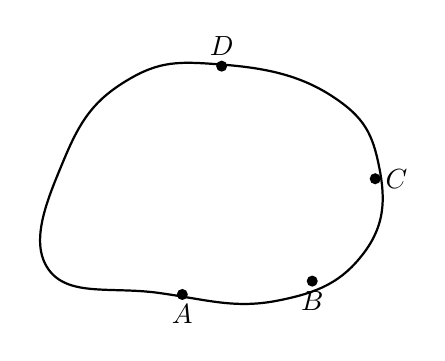
\begin{tikzpicture}[scale=1.0,thick]
\draw plot[smooth cycle,tension=.75] coordinates {(-2.2,-0.4) (-2.0,1.0) (-1.2,2.0) (0.0,2.2) (1.4,1.8) (2.0,0.9) (1.8,-0.2) (0.7,-0.8) (-0.8,-0.7)};
\fill (-0.5,-0.72) circle (2pt) node[below]{$A$};
\fill (1.15,-0.55) circle (2pt) node[below]{$B$};
\fill (1.95,0.75) circle (2pt) node[right]{$C$};
\fill (0.0,2.18) circle (2pt) node[above]{$D$};
\end{tikzpicture}
\caption{van der Pauw 法测量电导率示意图}
\label{fig:van-der-pauw}
\end{figure}

我们考虑如何从数值上检验这个关系式。引入电势 $\phi$，在 $\Omega$ 上其满足 Laplace 方程
\[
\nabla^2\phi=0.
\]
在电极以外的边界 $\partial\Omega$ 上，没有电流流入流出，即电势法向导数为零：
\[
\bm n\cdot\nabla\phi=0.
\]
而对于有电流流入流出的电极，任取一条初末点均在边界上，且包含该电极的曲线 $C$，有
\[
\sigma d\int_C\bm n\cdot\nabla\phi\,\mathrm dl=\pm I.
\]

\originalpage{221}{206}
试分别对于如下情形进行数值离散化，求解 $R_{AB,CD}$ 和 $R_{AD,BC}$，并验证在数值精度内满足 (1) 式：
\begin{enumerate}
\item $\Omega$ 为一个边长分别为 3 和 2 的长方形，$A,B,C,D$ 分别为四个顶点。
\item $\Omega$ 为一个对顶点距离分别为 3 和 2 的菱形，$A,B,C,D$ 分别为四条边的中点。
\item $\Omega$ 为一个长轴为 3、短轴为 2 的椭圆，$A,B,C,D$ 分别为长短轴与边界的交点。
\item $\Omega$ 为一个由极坐标方程 $r=3+2\cos2\theta$ 所给出的曲线围成的区域，$A,B,C,D$ 分别为该曲线上 $\theta=0,3\pi/4,3\pi/2,5\pi/4$ 的四个点。
\end{enumerate}

注意，你可以通过求解通量场而不是电势场来处理这个问题，但请勿使用保角变换或类似方法直接将该问题简化成一个可解析求解的情形。

% R17 extends through source PDF scan p.221 / printed p.206, completing Chapter 5.
